\makeatletter \@ifundefined{rootpath}{% Manual to memoir http://mirrors.dotsrc.org/ctan/macros/latex/contrib/memoir/memman.pdf

%\documentclass[a4paper,12pt,fleqn,openany,twoside]{memoir} %two sides for printing
\documentclass[a4paper,12pt,fleqn,openany,oneside]{memoir} %one side for pdf
\usepackage[english]{babel}
\usepackage[utf8]{inputenc}
\usepackage{microtype}
\usepackage{paralist}

%Definitions
\usepackage{amsthm}
\theoremstyle{plain}
\newtheorem{thm}{Theorem}[chapter] % reset theorem numbering for each chapter
\theoremstyle{definition}
\newtheorem{defn}[thm]{Definition}


% Choses the depth of numerations
\setsecnumdepth{subsubsection}

% Choses the depth of toc
%\maxtocdepth{subsection}

% LaTeX logical statements
\usepackage{ifthen}

% Fancy space after use of e.g. command
\usepackage{xspace}

% Skips after paragraphs
\usepackage{parskip}

% Layout settings
\setlength{\parindent}{0cm}
\setlength{\parskip}{2ex plus 2ex} %kan udvides til f.eks: '2ex plus 2ex minus 0ex'

\sloppybottom

% Don't make a collection per default
\newcommand{\worksheetcollection}{false}

% Bibtex
\usepackage[square,numbers,sort,comma]{natbib}
%\usepackage{cite}
%\bibliographystyle{plainnat}
\bibliographystyle{IEEEtran}


% Fixmes
\usepackage{fixme}
\fxsetup{draft}

% Mathematic
\usepackage{amsmath}
\usepackage{amsfonts}
\usepackage{amssymb}
\usepackage{stmaryrd}
\allowdisplaybreaks[1]


% Acronyms
\usepackage[printonlyused]{acronym}

% Images
\usepackage{graphicx}
\usepackage{wrapfig}
\usepackage[outdir=./]{epstopdf}
\usepackage{epsfig}


% Captions ans subcaptions
\captionnamefont{\footnotesize\bfseries}
\captiontitlefont{\footnotesize}

% Enable memoir subfloats for figures and tables
\newsubfloat{figure}
\newsubfloat{table}

% Hack memoir subfigure styles to have bold label and footnotesize fonts
\renewcommand{\thesubfigure}{\footnotesize\bfseries{(\alph{subfigure})}}
\renewcommand{\thesubtable}{\footnotesize\bfseries{(\alph{subtable})}}

\renewcommand{\subcaption}[2][]{\subbottom[\footnotesize{#1}]{#2}}

% Memoir tweak pagenumbers
%\pagestyle{headings}

% Tikz
\usepackage{tikz}
\usetikzlibrary{arrows,shapes,calc,positioning}
\pgfmathsetseed{1}

%Pgf plots
\usepackage{pgfplots}
\pgfplotsset{compat=1.5}
% loatbarrier, keep figures within (sub,subsub) sections
\usepackage{placeins}
\usepackage{pgfplots}
\usepgfplotslibrary{units}
\usepackage[space-before-unit,range-units = repeat]{siunitx}

% Hyperlinked auto references
\usepackage[hidelinks]{hyperref}
\usepackage[nameinlink]{cleveref}
\crefname{lstlisting}{Listing}{Listings}  
\Crefname{lstlisting}{Listing}{Listings}

\crefname{thm}{definition}{definitions}
\Crefname{thm}{Definition}{Definitions}

%\def\chapterautorefname{Kapitel}
%\def\sectionautorefname{Afsnit}
%\def\subsectionautorefname{Afsnit}
%\def\subsubsectionautorefname{Underafsnit}
%\def\figureautorefname{Figur}
%\def\lstlistingautorefname{Listing}
%\def\lstnumberautorefname{Linje}
%\def\itemautorefname{Punkt}
\usepackage[hypcap]{caption} % Link to top of the figure and not the caption

%Sick shit to make \Autoref command
%http://tex.stackexchange.com/questions/36575/autorefs-inserted-text-has-not-the-correct-case
\def\HyLang@english{%
  \def\equationautorefname{Equation}%
  \def\footnoteautorefname{Footnote}%
  \def\itemautorefname{item}%
  \def\figureautorefname{Figure}%
  \def\tableautorefname{Table}%
  \def\partautorefname{Part}%
  \def\appendixautorefname{Appendix}%
  \def\chapterautorefname{Chapter}%
  \def\sectionautorefname{Section}%
  \def\subsectionautorefname{Subsection}%
  \def\subsubsectionautorefname{Subsubsection}%
  \def\paragraphautorefname{Paragraph}%
  \def\subparagraphautorefname{Subparagraph}%
  \def\FancyVerbLineautorefname{Line}%
  \def\theoremautorefname{Theorem}%
  \def\pageautorefname{Page}%
}

% Reference greencommentssections with number and name
\usepackage{nameref}
\newcommand{\bsnameref}[1]{\Cref{#1} ``\nameref{#1}''}
\newcommand{\bsref}[1]{\Cref{#1}}
\newcommand{\bsbilagref}[1]{Appendix \ref{#1}}
\newcommand{\bsbilagnameref}[1]{Appendix \ref{#1} ``\nameref{#1}''}
\newcommand{\pling}[1]{``#1''}


% Listings for code qoutes
\usepackage{listings}
%\usepackage[usenames,dvipsnames,svgnames,table]{xcolor}
\usepackage{color}
\usepackage{xcolor}
\definecolor{bluekeywords}{rgb}{0.13,0.13,1}
\definecolor{greencomments}{rgb}{0,0.5,0}
\definecolor{redstrings}{rgb}{0.9,0,0}
\usepackage{caption} 
\usepackage{multicol}
\DeclareCaptionFont{white}{\color{white}}
\DeclareCaptionFormat{listing}{\colorbox{gray}{\parbox{\textwidth}{#1#2#3}}}
\captionsetup[lstlisting]{format=listing,labelfont=white,textfont=white}
%\lstset{numbers=left}
\lstset{
	basicstyle=\footnotesize,
	tabsize=2,
	breaklines=true,
  literate={æ}{{\ae}}1 {ø}{{\o}}1 {å}{{\aa}}1 {Æ}{{\AE}}1 {Ø}{{\O}}1 {Å}{{\AA}}1,
  keywords={typeof, new, true, false, catch, function, return, null, catch, switch, var, if, in, while, do, else, case, break},
  keywordstyle=\color{blue}\bfseries,
  ndkeywords={class, export, boolean, throw, implements, import, this},
  ndkeywordstyle=\color{darkgray}\bfseries,
  identifierstyle=\color{black},
  sensitive=false,
  comment=[l]{//},
  morecomment=[s]{/*}{*/},
  commentstyle=\color{purple}\ttfamily,
  stringstyle=\color{red}\ttfamily,
  numbers=left,
  numbersep=-5pt,
  showstringspaces=false,
  showspaces=false,
  %morestring=[b]',
  %morestring=[b]"
}
\lstnewenvironment{code}[1][]%
  {\minipage{\linewidth} 
   \lstset{basicstyle=\ttfamily\footnotesize,frame=single,#1}}
  {\endminipage}

\lstdefinelanguage{scala}{
  morekeywords={abstract,case,catch,class,def,%
    do,else,extends,false,final,finally,%
    for,if,implicit,import,match,mixin,%
    new,null,object,override,package,%
    private,protected,requires,return,sealed,%
    super,this,throw,trait,true,try,%
    type,val,var,while,with,yield, Unit, Boolean, Int},
  otherkeywords={=>,<-,<\%,<:,>:,\#,@},
  sensitive=true,
  morecomment=[l]{//},
  morecomment=[n]{/*}{*/},
  morestring=[b]",
  morestring=[b]',
  morestring=[b]"""
}

\lstdefinelanguage{clojure}%
{morekeywords={*,*1,*2,*3,*agent*,*allow-unresolved-vars*,*assert*,*clojure-version*,*command-line-args*,%
*compile-files*,*compile-path*,*e,*err*,*file*,*flush-on-newline*,*in*,*macro-meta*,%
*math-context*,*ns*,*out*,*print-dup*,*print-length*,*print-level*,*print-meta*,*print-readably*,%
*read-eval*,*source-path*,*use-context-classloader*,*warn-on-reflection*,+,-,->,->>,..,/,:else,%
<,<=,=,==,>,>=,@,accessor,aclone,add-classpath,add-watch,agent,agent-errors,aget,alength,alias,%
all-ns,alter,alter-meta!,alter-var-root,amap,ancestors,and,apply,areduce,array-map,aset,%
aset-boolean,aset-byte,aset-char,aset-double,aset-float,aset-int,aset-long,aset-short,assert,%
assoc,assoc!,assoc-in,associative?,atom,await,await-for,await1,bases,bean,bigdec,bigint,binding,%
bit-and,bit-and-not,bit-clear,bit-flip,bit-not,bit-or,bit-set,bit-shift-left,bit-shift-right,%
bit-test,bit-xor,boolean,boolean-array,booleans,bound-fn,bound-fn*,butlast,byte,byte-array,%
bytes,cast,char,char-array,char-escape-string,char-name-string,char?,chars,chunk,chunk-append,%
chunk-buffer,chunk-cons,chunk-first,chunk-next,chunk-rest,chunked-seq?,class,class?,%
clear-agent-errors,clojure-version,coll?,comment,commute,comp,comparator,compare,compare-and-set!,%
compile,complement,concat,cond,condp,conj,conj!,cons,constantly,construct-proxy,contains?,count,%
counted?,create-ns,create-struct,cycle,dec,decimal?,declare,def,definline,defmacro,defmethod,%
defmulti,defn,defn-,defonce,defprotocol,defstruct,deftype,delay,delay?,deliver,deref,derive,%
descendants,destructure,disj,disj!,dissoc,dissoc!,distinct,distinct?,do,do-template,doall,doc,%
dorun,doseq,dosync,dotimes,doto,double,double-array,doubles,drop,drop-last,drop-while,empty,empty?,%
ensure,enumeration-seq,eval,even?,every?,false,false?,ffirst,file-seq,filter,finally,find,find-doc,%
find-ns,find-var,first,float,float-array,float?,floats,flush,fn,fn?,fnext,for,force,format,future,%
future-call,future-cancel,future-cancelled?,future-done?,future?,gen-class,gen-interface,gensym,%
get,get-in,get-method,get-proxy-class,get-thread-bindings,get-validator,hash,hash-map,hash-set,%
identical?,identity,if,if-let,if-not,ifn?,import,in-ns,inc,init-proxy,instance?,int,int-array,%
integer?,interleave,intern,interpose,into,into-array,ints,io!,isa?,iterate,iterator-seq,juxt,%
key,keys,keyword,keyword?,last,lazy-cat,lazy-seq,let,letfn,line-seq,list,list*,list?,load,load-file,%
load-reader,load-string,loaded-libs,locking,long,long-array,longs,loop,macroexpand,macroexpand-1,%
make-array,make-hierarchy,map,map?,mapcat,max,max-key,memfn,memoize,merge,merge-with,meta,%
method-sig,methods,min,min-key,mod,monitor-enter,monitor-exit,name,namespace,neg?,new,newline,%
next,nfirst,nil,nil?,nnext,not,not-any?,not-empty,not-every?,not=,ns,ns-aliases,ns-imports,%
ns-interns,ns-map,ns-name,ns-publics,ns-refers,ns-resolve,ns-unalias,ns-unmap,nth,nthnext,num,%
number?,odd?,or,parents,partial,partition,pcalls,peek,persistent!,pmap,pop,pop!,pop-thread-bindings,%
pos?,pr,pr-str,prefer-method,prefers,primitives-classnames,print,print-ctor,print-doc,print-dup,%
print-method,print-namespace-doc,print-simple,print-special-doc,print-str,printf,println,println-str,%
prn,prn-str,promise,proxy,proxy-call-with-super,proxy-mappings,proxy-name,proxy-super,%
push-thread-bindings,pvalues,quot,rand,rand-int,range,ratio?,rational?,rationalize,re-find,%
re-groups,re-matcher,re-matches,re-pattern,re-seq,read,read-line,read-string,recur,reduce,ref,%
ref-history-count,ref-max-history,ref-min-history,ref-set,refer,refer-clojure,reify,%
release-pending-sends,rem,remove,remove-method,remove-ns,remove-watch,repeat,repeatedly,%
replace,replicate,require,reset!,reset-meta!,resolve,rest,resultset-seq,reverse,reversible?,%
rseq,rsubseq,second,select-keys,send,send-off,seq,seq?,seque,sequence,sequential?,set,set!,%
set-validator!,set?,short,short-array,shorts,shutdown-agents,slurp,some,sort,sort-by,sorted-map,%
sorted-map-by,sorted-set,sorted-set-by,sorted?,special-form-anchor,special-symbol?,split-at,%
split-with,str,stream?,string?,struct,struct-map,subs,subseq,subvec,supers,swap!,symbol,symbol?,%
sync,syntax-symbol-anchor,take,take-last,take-nth,take-while,test,the-ns,throw,time,to-array,%
to-array-2d,trampoline,transient,tree-seq,true,true?,try,type,unchecked-add,unchecked-dec,%
unchecked-divide,unchecked-inc,unchecked-multiply,unchecked-negate,unchecked-remainder,%
unchecked-subtract,underive,unquote,unquote-splicing,update-in,update-proxy,use,val,vals,%
var,var-get,var-set,var?,vary-meta,vec,vector,vector?,when,when-first,when-let,when-not,%
while,with-bindings,with-bindings*,with-in-str,with-loading-context,with-local-vars,%
with-meta,with-open,with-out-str,with-precision,xml-seq,zero?,zipmap
},%
   sensitive,% ???
   alsodigit=-,%
   morecomment=[l];,%
   morestring=[b]"%
  }[keywords,comments,strings]%

% Worksheet commands
\newcommand{\worksheetstart}[5]{ %Title, Revision, Date, Author, rootpath
	\ifthenelse{\equal{\worksheetcollection}{false}}{
		\newcommand{\rootpath}{#5}
		\documentheader
		\chapter{#1}
	}{
		\chapter{#1}
	}
%	\vspace{-1em}
%	\textbf{\tiny Revision #2 at #3. Written by #4}\\
%	\textbf{\tiny Hovedansvarlig #4}\\
%	\vspace{2em}\\
}

\newcommand{\worksheetend}{
	\ifthenelse{\equal{\worksheetcollection}{false}}{
		\collectionend
	}{}
}

\newcommand{\documentheader}{
	% Draws a tikz camera
% #1 is the coordinate to the top left corner
% #2 is a label for the righthand center position
% #3 is the text shown in the center of the camera
\newcommand{\camera}[3]{
\coordinate (anchor) at #1;
\draw (anchor) -- ($ (anchor) + (0em,-20pt) $) -- ($ (anchor) + (10pt, -15pt) $) -- ($ (anchor) + (10pt,-5pt)$) -- cycle;
\draw ($ (anchor) + (10pt,-5pt) $) -- ($ (anchor) + (10pt,0pt) $) -- ($ (anchor) + (50pt,0pt) $) -- ($ (anchor) + (50pt,-20pt) $) -- node[yshift=10pt] {\tiny #3} ($ (anchor) + (10pt,-20pt) $)-- cycle;
\coordinate (#2) at ($ (anchor) + (50pt,-10pt) $);
}

\newcounter{frameNumber}
\newcommand{\frameWithSize}[3][false]{
	\stepcounter{frameNumber}
	\coordinate (anchor) at #2;
	\ifthenelse{\equal{#1}{false}}{
		\def\frameNumber{\arabic{frameNumber}}
	}{
		\def\frameNumber{#1}
	}
	\pgfmathtruncatemacro\randomnumber{random(0,4)}
	\node[yshift=20pt] at (anchor) {\frameNumber};
	\ifthenelse{\equal{#3}{I}}{
		\node[draw, minimum size=20pt, fill=green!60] at (anchor) {I};
		\filldraw[fill=gray] ($(anchor) + (-10pt,-40pt)$) rectangle ($(anchor) + (10pt,-20pt) + (0pt,\randomnumber pt)$);
	}{
		\ifthenelse{\equal{#3}{P}}{
			\node[draw, minimum size=20pt, fill=yellow!60] at (anchor) {P};
			\filldraw[fill=gray] ($(anchor) + (-10pt,-40pt)$) rectangle ($(anchor) + (10pt,-30pt) + (0pt,\randomnumber pt)$);
		}{
			\node[draw, minimum size=20pt, fill=blue!40!yellow!60!black] at (anchor) {\color{white}B};
			\filldraw[fill=gray] ($(anchor) + (-10pt,-40pt)$) rectangle ($(anchor) + (10pt,-37pt) + (0pt,\randomnumber pt)$);
		}
	}
	\draw[thick] ($(anchor) + (-10pt,-40pt)$) -- +(20pt,0pt);
}

	\begin{document}
	%\renewcommand{\chaptername}{Worksheet}
	\chapterstyle{section}
	\renewcommand{\beforechapskip}{0pt}
	\renewcommand{\afterchapskip}{0pt}
}

\newcommand{\collectionstart}[1]{
	\newcommand{\rootpath}{#1}
	\renewcommand{\worksheetcollection}{true}
	\documentheader
	\frontmatter
	%\forside
	\makeatletter \@ifundefined{rootpath}{% Manual to memoir http://mirrors.dotsrc.org/ctan/macros/latex/contrib/memoir/memman.pdf

%\documentclass[a4paper,12pt,fleqn,openany,twoside]{memoir} %two sides for printing
\documentclass[a4paper,12pt,fleqn,openany,oneside]{memoir} %one side for pdf
\usepackage[english]{babel}
\usepackage[utf8]{inputenc}
\usepackage{microtype}
\usepackage{paralist}

%Definitions
\usepackage{amsthm}
\theoremstyle{plain}
\newtheorem{thm}{Theorem}[chapter] % reset theorem numbering for each chapter
\theoremstyle{definition}
\newtheorem{defn}[thm]{Definition}


% Choses the depth of numerations
\setsecnumdepth{subsubsection}

% Choses the depth of toc
%\maxtocdepth{subsection}

% LaTeX logical statements
\usepackage{ifthen}

% Fancy space after use of e.g. command
\usepackage{xspace}

% Skips after paragraphs
\usepackage{parskip}

% Layout settings
\setlength{\parindent}{0cm}
\setlength{\parskip}{2ex plus 2ex} %kan udvides til f.eks: '2ex plus 2ex minus 0ex'

\sloppybottom

% Don't make a collection per default
\newcommand{\worksheetcollection}{false}

% Bibtex
\usepackage[square,numbers,sort,comma]{natbib}
%\usepackage{cite}
%\bibliographystyle{plainnat}
\bibliographystyle{IEEEtran}


% Fixmes
\usepackage{fixme}
\fxsetup{draft}

% Mathematic
\usepackage{amsmath}
\usepackage{amsfonts}
\usepackage{amssymb}
\usepackage{stmaryrd}
\allowdisplaybreaks[1]


% Acronyms
\usepackage[printonlyused]{acronym}

% Images
\usepackage{graphicx}
\usepackage{wrapfig}
\usepackage[outdir=./]{epstopdf}
\usepackage{epsfig}


% Captions ans subcaptions
\captionnamefont{\footnotesize\bfseries}
\captiontitlefont{\footnotesize}

% Enable memoir subfloats for figures and tables
\newsubfloat{figure}
\newsubfloat{table}

% Hack memoir subfigure styles to have bold label and footnotesize fonts
\renewcommand{\thesubfigure}{\footnotesize\bfseries{(\alph{subfigure})}}
\renewcommand{\thesubtable}{\footnotesize\bfseries{(\alph{subtable})}}

\renewcommand{\subcaption}[2][]{\subbottom[\footnotesize{#1}]{#2}}

% Memoir tweak pagenumbers
%\pagestyle{headings}

% Tikz
\usepackage{tikz}
\usetikzlibrary{arrows,shapes,calc,positioning}
\pgfmathsetseed{1}

%Pgf plots
\usepackage{pgfplots}
\pgfplotsset{compat=1.5}
% loatbarrier, keep figures within (sub,subsub) sections
\usepackage{placeins}
\usepackage{pgfplots}
\usepgfplotslibrary{units}
\usepackage[space-before-unit,range-units = repeat]{siunitx}

% Hyperlinked auto references
\usepackage[hidelinks]{hyperref}
\usepackage[nameinlink]{cleveref}
\crefname{lstlisting}{Listing}{Listings}  
\Crefname{lstlisting}{Listing}{Listings}

\crefname{thm}{definition}{definitions}
\Crefname{thm}{Definition}{Definitions}

%\def\chapterautorefname{Kapitel}
%\def\sectionautorefname{Afsnit}
%\def\subsectionautorefname{Afsnit}
%\def\subsubsectionautorefname{Underafsnit}
%\def\figureautorefname{Figur}
%\def\lstlistingautorefname{Listing}
%\def\lstnumberautorefname{Linje}
%\def\itemautorefname{Punkt}
\usepackage[hypcap]{caption} % Link to top of the figure and not the caption

%Sick shit to make \Autoref command
%http://tex.stackexchange.com/questions/36575/autorefs-inserted-text-has-not-the-correct-case
\def\HyLang@english{%
  \def\equationautorefname{Equation}%
  \def\footnoteautorefname{Footnote}%
  \def\itemautorefname{item}%
  \def\figureautorefname{Figure}%
  \def\tableautorefname{Table}%
  \def\partautorefname{Part}%
  \def\appendixautorefname{Appendix}%
  \def\chapterautorefname{Chapter}%
  \def\sectionautorefname{Section}%
  \def\subsectionautorefname{Subsection}%
  \def\subsubsectionautorefname{Subsubsection}%
  \def\paragraphautorefname{Paragraph}%
  \def\subparagraphautorefname{Subparagraph}%
  \def\FancyVerbLineautorefname{Line}%
  \def\theoremautorefname{Theorem}%
  \def\pageautorefname{Page}%
}

% Reference greencommentssections with number and name
\usepackage{nameref}
\newcommand{\bsnameref}[1]{\Cref{#1} ``\nameref{#1}''}
\newcommand{\bsref}[1]{\Cref{#1}}
\newcommand{\bsbilagref}[1]{Appendix \ref{#1}}
\newcommand{\bsbilagnameref}[1]{Appendix \ref{#1} ``\nameref{#1}''}
\newcommand{\pling}[1]{``#1''}


% Listings for code qoutes
\usepackage{listings}
%\usepackage[usenames,dvipsnames,svgnames,table]{xcolor}
\usepackage{color}
\usepackage{xcolor}
\definecolor{bluekeywords}{rgb}{0.13,0.13,1}
\definecolor{greencomments}{rgb}{0,0.5,0}
\definecolor{redstrings}{rgb}{0.9,0,0}
\usepackage{caption} 
\usepackage{multicol}
\DeclareCaptionFont{white}{\color{white}}
\DeclareCaptionFormat{listing}{\colorbox{gray}{\parbox{\textwidth}{#1#2#3}}}
\captionsetup[lstlisting]{format=listing,labelfont=white,textfont=white}
%\lstset{numbers=left}
\lstset{
	basicstyle=\footnotesize,
	tabsize=2,
	breaklines=true,
  literate={æ}{{\ae}}1 {ø}{{\o}}1 {å}{{\aa}}1 {Æ}{{\AE}}1 {Ø}{{\O}}1 {Å}{{\AA}}1,
  keywords={typeof, new, true, false, catch, function, return, null, catch, switch, var, if, in, while, do, else, case, break},
  keywordstyle=\color{blue}\bfseries,
  ndkeywords={class, export, boolean, throw, implements, import, this},
  ndkeywordstyle=\color{darkgray}\bfseries,
  identifierstyle=\color{black},
  sensitive=false,
  comment=[l]{//},
  morecomment=[s]{/*}{*/},
  commentstyle=\color{purple}\ttfamily,
  stringstyle=\color{red}\ttfamily,
  numbers=left,
  numbersep=-5pt,
  showstringspaces=false,
  showspaces=false,
  %morestring=[b]',
  %morestring=[b]"
}
\lstnewenvironment{code}[1][]%
  {\minipage{\linewidth} 
   \lstset{basicstyle=\ttfamily\footnotesize,frame=single,#1}}
  {\endminipage}

\lstdefinelanguage{scala}{
  morekeywords={abstract,case,catch,class,def,%
    do,else,extends,false,final,finally,%
    for,if,implicit,import,match,mixin,%
    new,null,object,override,package,%
    private,protected,requires,return,sealed,%
    super,this,throw,trait,true,try,%
    type,val,var,while,with,yield, Unit, Boolean, Int},
  otherkeywords={=>,<-,<\%,<:,>:,\#,@},
  sensitive=true,
  morecomment=[l]{//},
  morecomment=[n]{/*}{*/},
  morestring=[b]",
  morestring=[b]',
  morestring=[b]"""
}

\lstdefinelanguage{clojure}%
{morekeywords={*,*1,*2,*3,*agent*,*allow-unresolved-vars*,*assert*,*clojure-version*,*command-line-args*,%
*compile-files*,*compile-path*,*e,*err*,*file*,*flush-on-newline*,*in*,*macro-meta*,%
*math-context*,*ns*,*out*,*print-dup*,*print-length*,*print-level*,*print-meta*,*print-readably*,%
*read-eval*,*source-path*,*use-context-classloader*,*warn-on-reflection*,+,-,->,->>,..,/,:else,%
<,<=,=,==,>,>=,@,accessor,aclone,add-classpath,add-watch,agent,agent-errors,aget,alength,alias,%
all-ns,alter,alter-meta!,alter-var-root,amap,ancestors,and,apply,areduce,array-map,aset,%
aset-boolean,aset-byte,aset-char,aset-double,aset-float,aset-int,aset-long,aset-short,assert,%
assoc,assoc!,assoc-in,associative?,atom,await,await-for,await1,bases,bean,bigdec,bigint,binding,%
bit-and,bit-and-not,bit-clear,bit-flip,bit-not,bit-or,bit-set,bit-shift-left,bit-shift-right,%
bit-test,bit-xor,boolean,boolean-array,booleans,bound-fn,bound-fn*,butlast,byte,byte-array,%
bytes,cast,char,char-array,char-escape-string,char-name-string,char?,chars,chunk,chunk-append,%
chunk-buffer,chunk-cons,chunk-first,chunk-next,chunk-rest,chunked-seq?,class,class?,%
clear-agent-errors,clojure-version,coll?,comment,commute,comp,comparator,compare,compare-and-set!,%
compile,complement,concat,cond,condp,conj,conj!,cons,constantly,construct-proxy,contains?,count,%
counted?,create-ns,create-struct,cycle,dec,decimal?,declare,def,definline,defmacro,defmethod,%
defmulti,defn,defn-,defonce,defprotocol,defstruct,deftype,delay,delay?,deliver,deref,derive,%
descendants,destructure,disj,disj!,dissoc,dissoc!,distinct,distinct?,do,do-template,doall,doc,%
dorun,doseq,dosync,dotimes,doto,double,double-array,doubles,drop,drop-last,drop-while,empty,empty?,%
ensure,enumeration-seq,eval,even?,every?,false,false?,ffirst,file-seq,filter,finally,find,find-doc,%
find-ns,find-var,first,float,float-array,float?,floats,flush,fn,fn?,fnext,for,force,format,future,%
future-call,future-cancel,future-cancelled?,future-done?,future?,gen-class,gen-interface,gensym,%
get,get-in,get-method,get-proxy-class,get-thread-bindings,get-validator,hash,hash-map,hash-set,%
identical?,identity,if,if-let,if-not,ifn?,import,in-ns,inc,init-proxy,instance?,int,int-array,%
integer?,interleave,intern,interpose,into,into-array,ints,io!,isa?,iterate,iterator-seq,juxt,%
key,keys,keyword,keyword?,last,lazy-cat,lazy-seq,let,letfn,line-seq,list,list*,list?,load,load-file,%
load-reader,load-string,loaded-libs,locking,long,long-array,longs,loop,macroexpand,macroexpand-1,%
make-array,make-hierarchy,map,map?,mapcat,max,max-key,memfn,memoize,merge,merge-with,meta,%
method-sig,methods,min,min-key,mod,monitor-enter,monitor-exit,name,namespace,neg?,new,newline,%
next,nfirst,nil,nil?,nnext,not,not-any?,not-empty,not-every?,not=,ns,ns-aliases,ns-imports,%
ns-interns,ns-map,ns-name,ns-publics,ns-refers,ns-resolve,ns-unalias,ns-unmap,nth,nthnext,num,%
number?,odd?,or,parents,partial,partition,pcalls,peek,persistent!,pmap,pop,pop!,pop-thread-bindings,%
pos?,pr,pr-str,prefer-method,prefers,primitives-classnames,print,print-ctor,print-doc,print-dup,%
print-method,print-namespace-doc,print-simple,print-special-doc,print-str,printf,println,println-str,%
prn,prn-str,promise,proxy,proxy-call-with-super,proxy-mappings,proxy-name,proxy-super,%
push-thread-bindings,pvalues,quot,rand,rand-int,range,ratio?,rational?,rationalize,re-find,%
re-groups,re-matcher,re-matches,re-pattern,re-seq,read,read-line,read-string,recur,reduce,ref,%
ref-history-count,ref-max-history,ref-min-history,ref-set,refer,refer-clojure,reify,%
release-pending-sends,rem,remove,remove-method,remove-ns,remove-watch,repeat,repeatedly,%
replace,replicate,require,reset!,reset-meta!,resolve,rest,resultset-seq,reverse,reversible?,%
rseq,rsubseq,second,select-keys,send,send-off,seq,seq?,seque,sequence,sequential?,set,set!,%
set-validator!,set?,short,short-array,shorts,shutdown-agents,slurp,some,sort,sort-by,sorted-map,%
sorted-map-by,sorted-set,sorted-set-by,sorted?,special-form-anchor,special-symbol?,split-at,%
split-with,str,stream?,string?,struct,struct-map,subs,subseq,subvec,supers,swap!,symbol,symbol?,%
sync,syntax-symbol-anchor,take,take-last,take-nth,take-while,test,the-ns,throw,time,to-array,%
to-array-2d,trampoline,transient,tree-seq,true,true?,try,type,unchecked-add,unchecked-dec,%
unchecked-divide,unchecked-inc,unchecked-multiply,unchecked-negate,unchecked-remainder,%
unchecked-subtract,underive,unquote,unquote-splicing,update-in,update-proxy,use,val,vals,%
var,var-get,var-set,var?,vary-meta,vec,vector,vector?,when,when-first,when-let,when-not,%
while,with-bindings,with-bindings*,with-in-str,with-loading-context,with-local-vars,%
with-meta,with-open,with-out-str,with-precision,xml-seq,zero?,zipmap
},%
   sensitive,% ???
   alsodigit=-,%
   morecomment=[l];,%
   morestring=[b]"%
  }[keywords,comments,strings]%

% Worksheet commands
\newcommand{\worksheetstart}[5]{ %Title, Revision, Date, Author, rootpath
	\ifthenelse{\equal{\worksheetcollection}{false}}{
		\newcommand{\rootpath}{#5}
		\documentheader
		\chapter{#1}
	}{
		\chapter{#1}
	}
%	\vspace{-1em}
%	\textbf{\tiny Revision #2 at #3. Written by #4}\\
%	\textbf{\tiny Hovedansvarlig #4}\\
%	\vspace{2em}\\
}

\newcommand{\worksheetend}{
	\ifthenelse{\equal{\worksheetcollection}{false}}{
		\collectionend
	}{}
}

\newcommand{\documentheader}{
	\input{\rootpath/setup/tikz-commands.tex}
	\begin{document}
	%\renewcommand{\chaptername}{Worksheet}
	\chapterstyle{section}
	\renewcommand{\beforechapskip}{0pt}
	\renewcommand{\afterchapskip}{0pt}
}

\newcommand{\collectionstart}[1]{
	\newcommand{\rootpath}{#1}
	\renewcommand{\worksheetcollection}{true}
	\documentheader
	\frontmatter
	%\forside
	\input{\rootpath/worksheets/titlepage/titlepage}
	\input{\rootpath/worksheets/preface/preface}
	%\input{\rootpath/worksheets/forord/forord}
	\newpage
	\newpage
	\tableofcontents*
	\mainmatter
}

\newcommand{\collectionend}{
	\backmatter
	\chapter{List of Acronyms}\vspace{3em}
	\input{\rootpath/setup/acronyms}
	\bibliography{\rootpath/setup/bibliography}
	\end{document}
}


\newcommand{\bscode}{
	\lstinline
}

\newcommand{\bscodemath}[1]{
	\text{\lstinline|#1|}
}

\newcommand{\bsqoute}[2]{
	\begin{quote}
		\textit{``#1''}
		\begin{center}
			-- \emph{#2}
		\end{center}
	\end{quote}
}


\newcommand{\lag}{\langle}
\newcommand{\rag}{\rangle}
\newcommand{\besk}[1]{\ensuremath{\lag #1 \rag}}

\newcommand{\namedtodo}[5]
{
  \ifthenelse{\equal{#1}{}}
  {
    \todo[color=#4,caption=
    {\textbf{#3: } #2}]
    {\color{#5}\textbf{#3: }#2}
  }
  {
    \todo[color=#4,caption=
    {\textbf{#3: } #1}
    ,inline]
    {\color{#5}\textbf{#3: }#2}
  }
}
\newcommand{\andreas}[2][]{\namedtodo{#1}{#2}{Andreas}{blue!50!red!10}{black}}
\newcommand{\lone}[2][]{\namedtodo{#1}{#2}{Lone}{orange}{black}}
\definecolor{babypink}{rgb}{0.96, 0.76, 0.76}
\newcommand{\toby}[2][]{\namedtodo{#1}{#2}{Tobias}{babypink}{black}}
\newcommand{\kasper}[2][]{\namedtodo{#1}{#2}{Kasper}{green}{black}}

%multicol
\usepackage{multicol}

% todonotes
%\usepackage[disable]{todonotes} %For final report
\usepackage{todonotes} %For writing notes
\usepackage{fancyvrb}

%Loading AAU macro
\usepackage{lastpage}
%%%%%%%%%%%%%%%%%%%%%%%%%%%%%%%%%%%%%%%%%%%%%%%%
% Macros for the titlepage
%%%%%%%%%%%%%%%%%%%%%%%%%%%%%%%%%%%%%%%%%%%%%%%%
%Creates the aau titlepage
\newcommand{\aautitlepage}[3]{%
  {
    %set up various length
    \ifx\titlepageleftcolumnwidth\undefined
      \newlength{\titlepageleftcolumnwidth}
      \newlength{\titlepagerightcolumnwidth}
    \fi
    \setlength{\titlepageleftcolumnwidth}{0.5\textwidth-\tabcolsep}
    \setlength{\titlepagerightcolumnwidth}{\textwidth-2\tabcolsep-\titlepageleftcolumnwidth}
    %create title page
    \thispagestyle{empty}
    \noindent%
    \begin{tabular}{@{}ll@{}}
      \parbox{\titlepageleftcolumnwidth}{
        \iflanguage{danish}{%
          
\includegraphics[width=\titlepageleftcolumnwidth]{titlepage/figures/aau_logo_da}
        }{%
          
\includegraphics[width=\titlepageleftcolumnwidth]{titlepage/figures/aau_logo_en}
        }
      } &
      \parbox{\titlepagerightcolumnwidth}{\raggedleft\small
        #2
      }\bigskip\\
       #1 &
      \parbox[t]{\titlepagerightcolumnwidth}{%
      \textbf{Abstract:}\bigskip\par
        \fbox{\parbox{\titlepagerightcolumnwidth-2\fboxsep-2\fboxrule}{%
          #3
        }}
      }\\
    \end{tabular}
    \vfill  
    \clearpage
  }
}

% Environment for problem statements
% Can be auto referenced.
\newtheorem{problem}{Problem}
\def\problemautorefname{Problem}

%Create english project info
\newcommand{\englishprojectinfo}[6]{%
  \parbox[t]{\titlepageleftcolumnwidth}{
    \textbf{Title:}\\ #1\bigskip\par
    %\textbf{Theme:}\\ #2\bigskip\par
    \textbf{Project Period:}\\ #2\bigskip\par
    \textbf{Project Group:}\\ #3\bigskip\par
    \textbf{Participants:}\\ #4\bigskip\par
    \textbf{Supervisor:}\\ #5\bigskip\par
    %\textbf{Copies:} #6\bigskip\par
    \textbf{Page Numbers:} \pageref{LastPage}\bigskip\par
    \textbf{Date of Completion:}\\ #6
  }
}



%Create danish project info
%\newcommand{\danishprojectinfo}[7]{%
 % \parbox[t]{\titlepageleftcolumnwidth}{
 %   \textbf{Titel:}\\ #1\bigskip\par
%    %\textbf{Tema:}\\ #2\bigskip\par
%    \textbf{Projektperiode:}\\ #2\bigskip\par
%    \textbf{Projektgruppe:}\\ #4\bigskip\par
%    \textbf{Deltager(e):}\\ #5\bigskip\par
 %   \textbf{Vejleder(e):}\\ #6\bigskip\par
%    \textbf{Oplagstal:} #7\bigskip\par
   % \textbf{Sidetal:} \pageref{LastPage}\bigskip\par
  %  \textbf{Afleveringsdato:}\\ #8
 % }
%}
}\makeatother
%\worksheetstart{Titlepage}{0}{December 31, 2012}{../../}
\begin{titlingpage}
\aautitlepage{%
  \englishprojectinfo{
    Scalable webservices %title
  }{%
    Spring Semester 2014 %project period
  }{%
    it801f14  % project group
  }{%
    %list of group members
    Tobias Ugleholdt Hansen\\
    Andreas Pørtner Karlsen\\ 
    Kasper Breinholt Laurberg\\
  }{%
    %list of supervisors
     Lone 
  }{%
    \today % date of completion
  }%
}{%department and address
  \textbf{Department of Computer Science}\\
  Selma Lagerløfs Vej 300\\
  DK-9220 Aalborg Ø\\
  \href{http://www.cs.aau.dk}{http://www.cs.aau.dk}
}{% the abstract
Some nice abstract
}
\end{titlingpage}
	\makeatletter \@ifundefined{rootpath}{% Manual to memoir http://mirrors.dotsrc.org/ctan/macros/latex/contrib/memoir/memman.pdf

%\documentclass[a4paper,12pt,fleqn,openany,twoside]{memoir} %two sides for printing
\documentclass[a4paper,12pt,fleqn,openany,oneside]{memoir} %one side for pdf
\usepackage[english]{babel}
\usepackage[utf8]{inputenc}
\usepackage{microtype}
\usepackage{paralist}

%Definitions
\usepackage{amsthm}
\theoremstyle{plain}
\newtheorem{thm}{Theorem}[chapter] % reset theorem numbering for each chapter
\theoremstyle{definition}
\newtheorem{defn}[thm]{Definition}


% Choses the depth of numerations
\setsecnumdepth{subsubsection}

% Choses the depth of toc
%\maxtocdepth{subsection}

% LaTeX logical statements
\usepackage{ifthen}

% Fancy space after use of e.g. command
\usepackage{xspace}

% Skips after paragraphs
\usepackage{parskip}

% Layout settings
\setlength{\parindent}{0cm}
\setlength{\parskip}{2ex plus 2ex} %kan udvides til f.eks: '2ex plus 2ex minus 0ex'

\sloppybottom

% Don't make a collection per default
\newcommand{\worksheetcollection}{false}

% Bibtex
\usepackage[square,numbers,sort,comma]{natbib}
%\usepackage{cite}
%\bibliographystyle{plainnat}
\bibliographystyle{IEEEtran}


% Fixmes
\usepackage{fixme}
\fxsetup{draft}

% Mathematic
\usepackage{amsmath}
\usepackage{amsfonts}
\usepackage{amssymb}
\usepackage{stmaryrd}
\allowdisplaybreaks[1]


% Acronyms
\usepackage[printonlyused]{acronym}

% Images
\usepackage{graphicx}
\usepackage{wrapfig}
\usepackage[outdir=./]{epstopdf}
\usepackage{epsfig}


% Captions ans subcaptions
\captionnamefont{\footnotesize\bfseries}
\captiontitlefont{\footnotesize}

% Enable memoir subfloats for figures and tables
\newsubfloat{figure}
\newsubfloat{table}

% Hack memoir subfigure styles to have bold label and footnotesize fonts
\renewcommand{\thesubfigure}{\footnotesize\bfseries{(\alph{subfigure})}}
\renewcommand{\thesubtable}{\footnotesize\bfseries{(\alph{subtable})}}

\renewcommand{\subcaption}[2][]{\subbottom[\footnotesize{#1}]{#2}}

% Memoir tweak pagenumbers
%\pagestyle{headings}

% Tikz
\usepackage{tikz}
\usetikzlibrary{arrows,shapes,calc,positioning}
\pgfmathsetseed{1}

%Pgf plots
\usepackage{pgfplots}
\pgfplotsset{compat=1.5}
% loatbarrier, keep figures within (sub,subsub) sections
\usepackage{placeins}
\usepackage{pgfplots}
\usepgfplotslibrary{units}
\usepackage[space-before-unit,range-units = repeat]{siunitx}

% Hyperlinked auto references
\usepackage[hidelinks]{hyperref}
\usepackage[nameinlink]{cleveref}
\crefname{lstlisting}{Listing}{Listings}  
\Crefname{lstlisting}{Listing}{Listings}

\crefname{thm}{definition}{definitions}
\Crefname{thm}{Definition}{Definitions}

%\def\chapterautorefname{Kapitel}
%\def\sectionautorefname{Afsnit}
%\def\subsectionautorefname{Afsnit}
%\def\subsubsectionautorefname{Underafsnit}
%\def\figureautorefname{Figur}
%\def\lstlistingautorefname{Listing}
%\def\lstnumberautorefname{Linje}
%\def\itemautorefname{Punkt}
\usepackage[hypcap]{caption} % Link to top of the figure and not the caption

%Sick shit to make \Autoref command
%http://tex.stackexchange.com/questions/36575/autorefs-inserted-text-has-not-the-correct-case
\def\HyLang@english{%
  \def\equationautorefname{Equation}%
  \def\footnoteautorefname{Footnote}%
  \def\itemautorefname{item}%
  \def\figureautorefname{Figure}%
  \def\tableautorefname{Table}%
  \def\partautorefname{Part}%
  \def\appendixautorefname{Appendix}%
  \def\chapterautorefname{Chapter}%
  \def\sectionautorefname{Section}%
  \def\subsectionautorefname{Subsection}%
  \def\subsubsectionautorefname{Subsubsection}%
  \def\paragraphautorefname{Paragraph}%
  \def\subparagraphautorefname{Subparagraph}%
  \def\FancyVerbLineautorefname{Line}%
  \def\theoremautorefname{Theorem}%
  \def\pageautorefname{Page}%
}

% Reference greencommentssections with number and name
\usepackage{nameref}
\newcommand{\bsnameref}[1]{\Cref{#1} ``\nameref{#1}''}
\newcommand{\bsref}[1]{\Cref{#1}}
\newcommand{\bsbilagref}[1]{Appendix \ref{#1}}
\newcommand{\bsbilagnameref}[1]{Appendix \ref{#1} ``\nameref{#1}''}
\newcommand{\pling}[1]{``#1''}


% Listings for code qoutes
\usepackage{listings}
%\usepackage[usenames,dvipsnames,svgnames,table]{xcolor}
\usepackage{color}
\usepackage{xcolor}
\definecolor{bluekeywords}{rgb}{0.13,0.13,1}
\definecolor{greencomments}{rgb}{0,0.5,0}
\definecolor{redstrings}{rgb}{0.9,0,0}
\usepackage{caption} 
\usepackage{multicol}
\DeclareCaptionFont{white}{\color{white}}
\DeclareCaptionFormat{listing}{\colorbox{gray}{\parbox{\textwidth}{#1#2#3}}}
\captionsetup[lstlisting]{format=listing,labelfont=white,textfont=white}
%\lstset{numbers=left}
\lstset{
	basicstyle=\footnotesize,
	tabsize=2,
	breaklines=true,
  literate={æ}{{\ae}}1 {ø}{{\o}}1 {å}{{\aa}}1 {Æ}{{\AE}}1 {Ø}{{\O}}1 {Å}{{\AA}}1,
  keywords={typeof, new, true, false, catch, function, return, null, catch, switch, var, if, in, while, do, else, case, break},
  keywordstyle=\color{blue}\bfseries,
  ndkeywords={class, export, boolean, throw, implements, import, this},
  ndkeywordstyle=\color{darkgray}\bfseries,
  identifierstyle=\color{black},
  sensitive=false,
  comment=[l]{//},
  morecomment=[s]{/*}{*/},
  commentstyle=\color{purple}\ttfamily,
  stringstyle=\color{red}\ttfamily,
  numbers=left,
  numbersep=-5pt,
  showstringspaces=false,
  showspaces=false,
  %morestring=[b]',
  %morestring=[b]"
}
\lstnewenvironment{code}[1][]%
  {\minipage{\linewidth} 
   \lstset{basicstyle=\ttfamily\footnotesize,frame=single,#1}}
  {\endminipage}

\lstdefinelanguage{scala}{
  morekeywords={abstract,case,catch,class,def,%
    do,else,extends,false,final,finally,%
    for,if,implicit,import,match,mixin,%
    new,null,object,override,package,%
    private,protected,requires,return,sealed,%
    super,this,throw,trait,true,try,%
    type,val,var,while,with,yield, Unit, Boolean, Int},
  otherkeywords={=>,<-,<\%,<:,>:,\#,@},
  sensitive=true,
  morecomment=[l]{//},
  morecomment=[n]{/*}{*/},
  morestring=[b]",
  morestring=[b]',
  morestring=[b]"""
}

\lstdefinelanguage{clojure}%
{morekeywords={*,*1,*2,*3,*agent*,*allow-unresolved-vars*,*assert*,*clojure-version*,*command-line-args*,%
*compile-files*,*compile-path*,*e,*err*,*file*,*flush-on-newline*,*in*,*macro-meta*,%
*math-context*,*ns*,*out*,*print-dup*,*print-length*,*print-level*,*print-meta*,*print-readably*,%
*read-eval*,*source-path*,*use-context-classloader*,*warn-on-reflection*,+,-,->,->>,..,/,:else,%
<,<=,=,==,>,>=,@,accessor,aclone,add-classpath,add-watch,agent,agent-errors,aget,alength,alias,%
all-ns,alter,alter-meta!,alter-var-root,amap,ancestors,and,apply,areduce,array-map,aset,%
aset-boolean,aset-byte,aset-char,aset-double,aset-float,aset-int,aset-long,aset-short,assert,%
assoc,assoc!,assoc-in,associative?,atom,await,await-for,await1,bases,bean,bigdec,bigint,binding,%
bit-and,bit-and-not,bit-clear,bit-flip,bit-not,bit-or,bit-set,bit-shift-left,bit-shift-right,%
bit-test,bit-xor,boolean,boolean-array,booleans,bound-fn,bound-fn*,butlast,byte,byte-array,%
bytes,cast,char,char-array,char-escape-string,char-name-string,char?,chars,chunk,chunk-append,%
chunk-buffer,chunk-cons,chunk-first,chunk-next,chunk-rest,chunked-seq?,class,class?,%
clear-agent-errors,clojure-version,coll?,comment,commute,comp,comparator,compare,compare-and-set!,%
compile,complement,concat,cond,condp,conj,conj!,cons,constantly,construct-proxy,contains?,count,%
counted?,create-ns,create-struct,cycle,dec,decimal?,declare,def,definline,defmacro,defmethod,%
defmulti,defn,defn-,defonce,defprotocol,defstruct,deftype,delay,delay?,deliver,deref,derive,%
descendants,destructure,disj,disj!,dissoc,dissoc!,distinct,distinct?,do,do-template,doall,doc,%
dorun,doseq,dosync,dotimes,doto,double,double-array,doubles,drop,drop-last,drop-while,empty,empty?,%
ensure,enumeration-seq,eval,even?,every?,false,false?,ffirst,file-seq,filter,finally,find,find-doc,%
find-ns,find-var,first,float,float-array,float?,floats,flush,fn,fn?,fnext,for,force,format,future,%
future-call,future-cancel,future-cancelled?,future-done?,future?,gen-class,gen-interface,gensym,%
get,get-in,get-method,get-proxy-class,get-thread-bindings,get-validator,hash,hash-map,hash-set,%
identical?,identity,if,if-let,if-not,ifn?,import,in-ns,inc,init-proxy,instance?,int,int-array,%
integer?,interleave,intern,interpose,into,into-array,ints,io!,isa?,iterate,iterator-seq,juxt,%
key,keys,keyword,keyword?,last,lazy-cat,lazy-seq,let,letfn,line-seq,list,list*,list?,load,load-file,%
load-reader,load-string,loaded-libs,locking,long,long-array,longs,loop,macroexpand,macroexpand-1,%
make-array,make-hierarchy,map,map?,mapcat,max,max-key,memfn,memoize,merge,merge-with,meta,%
method-sig,methods,min,min-key,mod,monitor-enter,monitor-exit,name,namespace,neg?,new,newline,%
next,nfirst,nil,nil?,nnext,not,not-any?,not-empty,not-every?,not=,ns,ns-aliases,ns-imports,%
ns-interns,ns-map,ns-name,ns-publics,ns-refers,ns-resolve,ns-unalias,ns-unmap,nth,nthnext,num,%
number?,odd?,or,parents,partial,partition,pcalls,peek,persistent!,pmap,pop,pop!,pop-thread-bindings,%
pos?,pr,pr-str,prefer-method,prefers,primitives-classnames,print,print-ctor,print-doc,print-dup,%
print-method,print-namespace-doc,print-simple,print-special-doc,print-str,printf,println,println-str,%
prn,prn-str,promise,proxy,proxy-call-with-super,proxy-mappings,proxy-name,proxy-super,%
push-thread-bindings,pvalues,quot,rand,rand-int,range,ratio?,rational?,rationalize,re-find,%
re-groups,re-matcher,re-matches,re-pattern,re-seq,read,read-line,read-string,recur,reduce,ref,%
ref-history-count,ref-max-history,ref-min-history,ref-set,refer,refer-clojure,reify,%
release-pending-sends,rem,remove,remove-method,remove-ns,remove-watch,repeat,repeatedly,%
replace,replicate,require,reset!,reset-meta!,resolve,rest,resultset-seq,reverse,reversible?,%
rseq,rsubseq,second,select-keys,send,send-off,seq,seq?,seque,sequence,sequential?,set,set!,%
set-validator!,set?,short,short-array,shorts,shutdown-agents,slurp,some,sort,sort-by,sorted-map,%
sorted-map-by,sorted-set,sorted-set-by,sorted?,special-form-anchor,special-symbol?,split-at,%
split-with,str,stream?,string?,struct,struct-map,subs,subseq,subvec,supers,swap!,symbol,symbol?,%
sync,syntax-symbol-anchor,take,take-last,take-nth,take-while,test,the-ns,throw,time,to-array,%
to-array-2d,trampoline,transient,tree-seq,true,true?,try,type,unchecked-add,unchecked-dec,%
unchecked-divide,unchecked-inc,unchecked-multiply,unchecked-negate,unchecked-remainder,%
unchecked-subtract,underive,unquote,unquote-splicing,update-in,update-proxy,use,val,vals,%
var,var-get,var-set,var?,vary-meta,vec,vector,vector?,when,when-first,when-let,when-not,%
while,with-bindings,with-bindings*,with-in-str,with-loading-context,with-local-vars,%
with-meta,with-open,with-out-str,with-precision,xml-seq,zero?,zipmap
},%
   sensitive,% ???
   alsodigit=-,%
   morecomment=[l];,%
   morestring=[b]"%
  }[keywords,comments,strings]%

% Worksheet commands
\newcommand{\worksheetstart}[5]{ %Title, Revision, Date, Author, rootpath
	\ifthenelse{\equal{\worksheetcollection}{false}}{
		\newcommand{\rootpath}{#5}
		\documentheader
		\chapter{#1}
	}{
		\chapter{#1}
	}
%	\vspace{-1em}
%	\textbf{\tiny Revision #2 at #3. Written by #4}\\
%	\textbf{\tiny Hovedansvarlig #4}\\
%	\vspace{2em}\\
}

\newcommand{\worksheetend}{
	\ifthenelse{\equal{\worksheetcollection}{false}}{
		\collectionend
	}{}
}

\newcommand{\documentheader}{
	\input{\rootpath/setup/tikz-commands.tex}
	\begin{document}
	%\renewcommand{\chaptername}{Worksheet}
	\chapterstyle{section}
	\renewcommand{\beforechapskip}{0pt}
	\renewcommand{\afterchapskip}{0pt}
}

\newcommand{\collectionstart}[1]{
	\newcommand{\rootpath}{#1}
	\renewcommand{\worksheetcollection}{true}
	\documentheader
	\frontmatter
	%\forside
	\input{\rootpath/worksheets/titlepage/titlepage}
	\input{\rootpath/worksheets/preface/preface}
	%\input{\rootpath/worksheets/forord/forord}
	\newpage
	\newpage
	\tableofcontents*
	\mainmatter
}

\newcommand{\collectionend}{
	\backmatter
	\chapter{List of Acronyms}\vspace{3em}
	\input{\rootpath/setup/acronyms}
	\bibliography{\rootpath/setup/bibliography}
	\end{document}
}


\newcommand{\bscode}{
	\lstinline
}

\newcommand{\bscodemath}[1]{
	\text{\lstinline|#1|}
}

\newcommand{\bsqoute}[2]{
	\begin{quote}
		\textit{``#1''}
		\begin{center}
			-- \emph{#2}
		\end{center}
	\end{quote}
}


\newcommand{\lag}{\langle}
\newcommand{\rag}{\rangle}
\newcommand{\besk}[1]{\ensuremath{\lag #1 \rag}}

\newcommand{\namedtodo}[5]
{
  \ifthenelse{\equal{#1}{}}
  {
    \todo[color=#4,caption=
    {\textbf{#3: } #2}]
    {\color{#5}\textbf{#3: }#2}
  }
  {
    \todo[color=#4,caption=
    {\textbf{#3: } #1}
    ,inline]
    {\color{#5}\textbf{#3: }#2}
  }
}
\newcommand{\andreas}[2][]{\namedtodo{#1}{#2}{Andreas}{blue!50!red!10}{black}}
\newcommand{\lone}[2][]{\namedtodo{#1}{#2}{Lone}{orange}{black}}
\definecolor{babypink}{rgb}{0.96, 0.76, 0.76}
\newcommand{\toby}[2][]{\namedtodo{#1}{#2}{Tobias}{babypink}{black}}
\newcommand{\kasper}[2][]{\namedtodo{#1}{#2}{Kasper}{green}{black}}

%multicol
\usepackage{multicol}

% todonotes
%\usepackage[disable]{todonotes} %For final report
\usepackage{todonotes} %For writing notes
\usepackage{fancyvrb}

%Loading AAU macro
\usepackage{lastpage}
%%%%%%%%%%%%%%%%%%%%%%%%%%%%%%%%%%%%%%%%%%%%%%%%
% Macros for the titlepage
%%%%%%%%%%%%%%%%%%%%%%%%%%%%%%%%%%%%%%%%%%%%%%%%
%Creates the aau titlepage
\newcommand{\aautitlepage}[3]{%
  {
    %set up various length
    \ifx\titlepageleftcolumnwidth\undefined
      \newlength{\titlepageleftcolumnwidth}
      \newlength{\titlepagerightcolumnwidth}
    \fi
    \setlength{\titlepageleftcolumnwidth}{0.5\textwidth-\tabcolsep}
    \setlength{\titlepagerightcolumnwidth}{\textwidth-2\tabcolsep-\titlepageleftcolumnwidth}
    %create title page
    \thispagestyle{empty}
    \noindent%
    \begin{tabular}{@{}ll@{}}
      \parbox{\titlepageleftcolumnwidth}{
        \iflanguage{danish}{%
          
\includegraphics[width=\titlepageleftcolumnwidth]{titlepage/figures/aau_logo_da}
        }{%
          
\includegraphics[width=\titlepageleftcolumnwidth]{titlepage/figures/aau_logo_en}
        }
      } &
      \parbox{\titlepagerightcolumnwidth}{\raggedleft\small
        #2
      }\bigskip\\
       #1 &
      \parbox[t]{\titlepagerightcolumnwidth}{%
      \textbf{Abstract:}\bigskip\par
        \fbox{\parbox{\titlepagerightcolumnwidth-2\fboxsep-2\fboxrule}{%
          #3
        }}
      }\\
    \end{tabular}
    \vfill  
    \clearpage
  }
}

% Environment for problem statements
% Can be auto referenced.
\newtheorem{problem}{Problem}
\def\problemautorefname{Problem}

%Create english project info
\newcommand{\englishprojectinfo}[6]{%
  \parbox[t]{\titlepageleftcolumnwidth}{
    \textbf{Title:}\\ #1\bigskip\par
    %\textbf{Theme:}\\ #2\bigskip\par
    \textbf{Project Period:}\\ #2\bigskip\par
    \textbf{Project Group:}\\ #3\bigskip\par
    \textbf{Participants:}\\ #4\bigskip\par
    \textbf{Supervisor:}\\ #5\bigskip\par
    %\textbf{Copies:} #6\bigskip\par
    \textbf{Page Numbers:} \pageref{LastPage}\bigskip\par
    \textbf{Date of Completion:}\\ #6
  }
}



%Create danish project info
%\newcommand{\danishprojectinfo}[7]{%
 % \parbox[t]{\titlepageleftcolumnwidth}{
 %   \textbf{Titel:}\\ #1\bigskip\par
%    %\textbf{Tema:}\\ #2\bigskip\par
%    \textbf{Projektperiode:}\\ #2\bigskip\par
%    \textbf{Projektgruppe:}\\ #4\bigskip\par
%    \textbf{Deltager(e):}\\ #5\bigskip\par
 %   \textbf{Vejleder(e):}\\ #6\bigskip\par
%    \textbf{Oplagstal:} #7\bigskip\par
   % \textbf{Sidetal:} \pageref{LastPage}\bigskip\par
  %  \textbf{Afleveringsdato:}\\ #8
 % }
%}
}\makeatother
\worksheetstart{Preface}{1}{December 17, 2013}{Mino}{../../}
This report documents project work done by group dpt907e14 at the Department of Computer Science at Aalborg University. The report was written as part of the Computer Science (IT) study program in the fall of 2014.

\newpage
\vspace*{30 mm}
%\vspace*{\fill}
\begin{vplace}

\begin{minipage}[b]{0.45\textwidth}
 \centering
 \rule{\textwidth}{0.5pt}\\
  Tobias Ugleholdt Hansen\\
 {\footnotesize tuha13@student.aau.dk}
\end{minipage}
\begin{minipage}[b]{0.45\textwidth}
 \centering
 \rule{\textwidth}{0.5pt}\\
  Andreas Pørtner Karlsen\\
 {\footnotesize akarls13@student.aau.dk}
\end{minipage}\\\\
\begin{minipage}[b]{0.45\textwidth}
 \centering
 \rule{\textwidth}{0.5pt}\\
  Kasper Breinholt Laurberg\\
 {\footnotesize klaurb13@student.aau.dk}
\end{minipage}\\\\


\end{vplace}
\worksheetend

	%\input{\rootpath/worksheets/forord/forord}
	\newpage
	\newpage
	\tableofcontents*
	\mainmatter
}

\newcommand{\collectionend}{
	\backmatter
	\chapter{List of Acronyms}\vspace{3em}
	\begin{acronym}[ITU-T]
\acro{WS}{Webservice}
\acro{CPU}{Central Processing Unit}
\acrodefplural{CPU}[CPU's]{Central Processing Units}
\acro{STM}{Software Transactional Memory}
\acro{TL}{Threads \& Locks}
\acro{ACID}{Atomicity, Consistency, Isolation, Durability}
\acro{JVM}{Java Virtual Machine}
\acro{CLR}{Common Language Runtime}
\acro{FIFO}{First In First Out}
\acro{LIFO}{Last In First Out}
\acro{CSP}{Communicating Sequential Processes}
\acro{PCC}{Pearson Correlation Coefficient}
\acro{FRP}{Functional Reactive Programming}
\acro{FP}{Functional Programming}
\acro{Rx}{Reactive Extensions}
\acro{OS}{Operating System}
\acro{OOP}{Object Oriented Programming}
\end{acronym}

	\bibliography{\rootpath/setup/bibliography}
	\end{document}
}


\newcommand{\bscode}{
	\lstinline
}

\newcommand{\bscodemath}[1]{
	\text{\lstinline|#1|}
}

\newcommand{\bsqoute}[2]{
	\begin{quote}
		\textit{``#1''}
		\begin{center}
			-- \emph{#2}
		\end{center}
	\end{quote}
}


\newcommand{\lag}{\langle}
\newcommand{\rag}{\rangle}
\newcommand{\besk}[1]{\ensuremath{\lag #1 \rag}}

\newcommand{\namedtodo}[5]
{
  \ifthenelse{\equal{#1}{}}
  {
    \todo[color=#4,caption=
    {\textbf{#3: } #2}]
    {\color{#5}\textbf{#3: }#2}
  }
  {
    \todo[color=#4,caption=
    {\textbf{#3: } #1}
    ,inline]
    {\color{#5}\textbf{#3: }#2}
  }
}
\newcommand{\andreas}[2][]{\namedtodo{#1}{#2}{Andreas}{blue!50!red!10}{black}}
\newcommand{\lone}[2][]{\namedtodo{#1}{#2}{Lone}{orange}{black}}
\definecolor{babypink}{rgb}{0.96, 0.76, 0.76}
\newcommand{\toby}[2][]{\namedtodo{#1}{#2}{Tobias}{babypink}{black}}
\newcommand{\kasper}[2][]{\namedtodo{#1}{#2}{Kasper}{green}{black}}

%multicol
\usepackage{multicol}

% todonotes
%\usepackage[disable]{todonotes} %For final report
\usepackage{todonotes} %For writing notes
\usepackage{fancyvrb}

%Loading AAU macro
\usepackage{lastpage}
%%%%%%%%%%%%%%%%%%%%%%%%%%%%%%%%%%%%%%%%%%%%%%%%
% Macros for the titlepage
%%%%%%%%%%%%%%%%%%%%%%%%%%%%%%%%%%%%%%%%%%%%%%%%
%Creates the aau titlepage
\newcommand{\aautitlepage}[3]{%
  {
    %set up various length
    \ifx\titlepageleftcolumnwidth\undefined
      \newlength{\titlepageleftcolumnwidth}
      \newlength{\titlepagerightcolumnwidth}
    \fi
    \setlength{\titlepageleftcolumnwidth}{0.5\textwidth-\tabcolsep}
    \setlength{\titlepagerightcolumnwidth}{\textwidth-2\tabcolsep-\titlepageleftcolumnwidth}
    %create title page
    \thispagestyle{empty}
    \noindent%
    \begin{tabular}{@{}ll@{}}
      \parbox{\titlepageleftcolumnwidth}{
        \iflanguage{danish}{%
          
\includegraphics[width=\titlepageleftcolumnwidth]{titlepage/figures/aau_logo_da}
        }{%
          
\includegraphics[width=\titlepageleftcolumnwidth]{titlepage/figures/aau_logo_en}
        }
      } &
      \parbox{\titlepagerightcolumnwidth}{\raggedleft\small
        #2
      }\bigskip\\
       #1 &
      \parbox[t]{\titlepagerightcolumnwidth}{%
      \textbf{Abstract:}\bigskip\par
        \fbox{\parbox{\titlepagerightcolumnwidth-2\fboxsep-2\fboxrule}{%
          #3
        }}
      }\\
    \end{tabular}
    \vfill  
    \clearpage
  }
}

% Environment for problem statements
% Can be auto referenced.
\newtheorem{problem}{Problem}
\def\problemautorefname{Problem}

%Create english project info
\newcommand{\englishprojectinfo}[6]{%
  \parbox[t]{\titlepageleftcolumnwidth}{
    \textbf{Title:}\\ #1\bigskip\par
    %\textbf{Theme:}\\ #2\bigskip\par
    \textbf{Project Period:}\\ #2\bigskip\par
    \textbf{Project Group:}\\ #3\bigskip\par
    \textbf{Participants:}\\ #4\bigskip\par
    \textbf{Supervisor:}\\ #5\bigskip\par
    %\textbf{Copies:} #6\bigskip\par
    \textbf{Page Numbers:} \pageref{LastPage}\bigskip\par
    \textbf{Date of Completion:}\\ #6
  }
}



%Create danish project info
%\newcommand{\danishprojectinfo}[7]{%
 % \parbox[t]{\titlepageleftcolumnwidth}{
 %   \textbf{Titel:}\\ #1\bigskip\par
%    %\textbf{Tema:}\\ #2\bigskip\par
%    \textbf{Projektperiode:}\\ #2\bigskip\par
%    \textbf{Projektgruppe:}\\ #4\bigskip\par
%    \textbf{Deltager(e):}\\ #5\bigskip\par
 %   \textbf{Vejleder(e):}\\ #6\bigskip\par
%    \textbf{Oplagstal:} #7\bigskip\par
   % \textbf{Sidetal:} \pageref{LastPage}\bigskip\par
  %  \textbf{Afleveringsdato:}\\ #8
 % }
%}
}\makeatother
\worksheetstart{Software Transactional Memory}{1}{November 7, 2013}{Andreas}{../../}
This chapter investigates \ac{STM} as a concurrency model. In \bsref{sec:stm_keyconcepts}, the key concepts of \ac{STM} are described. \bsref{sec:stm_issues} documents the concurrency issues introduced by \ac{STM}. \bsref{sec:stm_discussion} discusses the properties of \ac{STM}. Finally, in \bsref{sec:stm_eval} an evaluation of \ac{STM} as a concurrency model is conducted.
\label{chap:stm}

\section{Key Concepts}
\label{sec:stm_keyconcepts}
This section presents the key concepts of \ac{STM}. It clarifies the concepts of \ac{STM}, so the discussion and comparison in the subsequent sections can be at a higher level of abstraction.

\subsection{\acl{TM}}
\label{sec:tmevo}
In \cite{herlihy1993transactional} the authors proposes a way to implement \ac{TM} at hardware level. Due to the inflexible properties of hardware, i.e. fixed instruction set and limited register size, \ac{TM} implemented on hardware is limited to existing instructions and can only handle transactions of limited size\cite{dragojevic2011stm}. This causes high implementation and verification costs\cite{cascaval2008software}. \ac{HTM} also exposes low level hardware details and limitations\cite{herlihy2011tm}, which preferably should be abstracted away from the programmer, to ensure semantic correctness of the transactions regardless of the hardware limitations. 

Due to these caveats, a software based solution is presented by \cite{shavit1997software}. This solution, entirely implemented as software, is known as \acl{STM}. Being implemented as a software solution, \ac{STM} does not suffer the same issues as \ac{HTM}, but still provides the transactional semantics. However, providing these semantics in software only, comes with a performance penalty\cite{cascaval2008software}\cite{dragojevic2011stm}.

Recently \ac{HTM} has been adopted by Intel and IBM and integrated into the Haswell and POWER8 processors respectively\cite{Anthes:2014:RSP:2684442.2667109}. Researchers hope to develop a hybrid model, which leverages the low level \ac{TM} instructions on the \ac{CPU} for good performance, while providing a transactional programming model to the developer at software level, to make the high level programming simpler, efficient, and well structured\cite{Anthes:2014:RSP:2684442.2667109}.

Despite the recent development in the area of \ac{HTM}, the availability of \ac{HTM} or hybrids in high level programming languages is to our best knowledge non-existent. One could speculate, that the programming model to the programmer will remain unchanged, but the underlying runtime will benefit from the new \ac{HTM} semantics available, and therefore the characteristics of the \ac{STM} programming model could be the same. Due to these observations, \ac{STM} is the focal point of our investigation in \ac{TM} as a concurrency mechanism. 

\subsection{Transactional Properties}
\label{sec:stm_tm_properties}
\ac{TM} is based on the concept of a transaction. A transaction is a finite sequence of machine instructions, executed by a single process, satisfying following properties\cite[p. 2]{herlihy2011tm}.

\paragraph{Atomicity} By considering the instructions in a transaction as indivisible, atomicity ensures a shared effect of all the instructions in the transactions, either success or failure. That is, either all the instructions succeed to change the state of the system or none of them take effect e.g. if a single instruction in a transaction fails, all will fail.
\paragraph{Isolation} A transaction is only perceived before or after its execution, never in the middle. That is, the work of a transaction can be perceived to occur instantaneously. This can be either from the view of the entire system, or other transactions. We will elaborate on this in \bsref{subsec:isolation_level}. 

\ac{TM} can perform a group of memory-operations atomically\cite[48]{harris2005composable}\toby{Den står lidt som et fact der ikke bliver bygget mere på, måske byg denne sætning sammen med næste eller uddyb}. By utilizing the transactional approach, \ac{TM} serves as a concurrency control mechanism. By adhering to the aforementioned properties, \ac{TM} enables concurrent execution, while being semantically equivalent to serial execution of the same program.

\subsection{\acl{STM}}\label{sec:stm_stm}
\ac{STM} provides programmers with a transactional model, in software, through a library or compiler interface\cite{herlihy2011tm}. It seeks to solve the issues introduced by running multiple processes concurrently in a shared memory space, e.g. race conditions as discussed in \bsref{subsec:race_coditions}. To handle these challenges, \ac{STM} offers the programmer ways to define transaction scopes in critical regions. The transactions are executed concurrently, and if successful, changes are committed. If the transactions are not successful, it will be retried. Just by defining the critical regions, the \ac{STM} takes care of ensuring the atomicity and isolation leaving no work left for the programmer. 

The example in \bsref{lst:stmexample} demonstrates a transaction in Clojure\andreas{Should reason about the choice for clojure now? Atm its in performance} on line 5, specified with the \bscode{dosync} function. Two accounts, \bscode{account1} and \bscode{account2} respectively, are defined as a reference to an amount. The function \bscode{transfer} takes an amount, and two accounts as parameters. In a transaction, it then transfers the amount given, from one account, to the other.

\begin{lstlisting}[label=lst:stmexample,
  caption={STM in Clojure},
  language=Lisp,  
  showspaces=false,
  showtabs=false,
  breaklines=true,
  showstringspaces=false,
  breakatwhitespace=true,
  commentstyle=\color{greencomments},
  keywordstyle=\color{bluekeywords},
  stringstyle=\color{redstrings}]  % Start your code-block

	(def account1 (ref 100))
	(def account2 (ref 0))

	(defn transfer [amount from to]
    	(dosync
    		(alter from - amount)
    		(alter to + amount)))
       
\end{lstlisting}

To clarify the effect of using \ac{STM}, \bsref{fig:transaction} visualizes the flow of an example of two transactions running concurrently. Both transactions \bscode{t1} and \bscode{t2} are in the same process, and therefore share memory. The variable \bscode{x} is stored in this memory. Both transactions have a reference to variable x. We use the concept of revisions of a variable, to describe how the value of it evolves. First off, both \bscode{t1} and \bscode{t2} are reading the initial value of x. They want to perform a statement to update the value of x, leading to a race condition. \bscode{t1} finishes its statement first, and wants to commit its transaction. This is allowed, since the revision of x is unchanged since the read. Afterwards, \bscode{t2} wants to commit its transaction. This is disallowed, since the revision of x now has increased. \bscode{t2} then retries its transaction, by re-reading the value of x, performing the statement again, and committing the transaction. This is now allowed, since x is the same revision as when it was read by \bscode{t2}. It is clear from the example given, that \ac{STM} remedied the risk of race conditions.

\begin{figure}[h!]
\centering
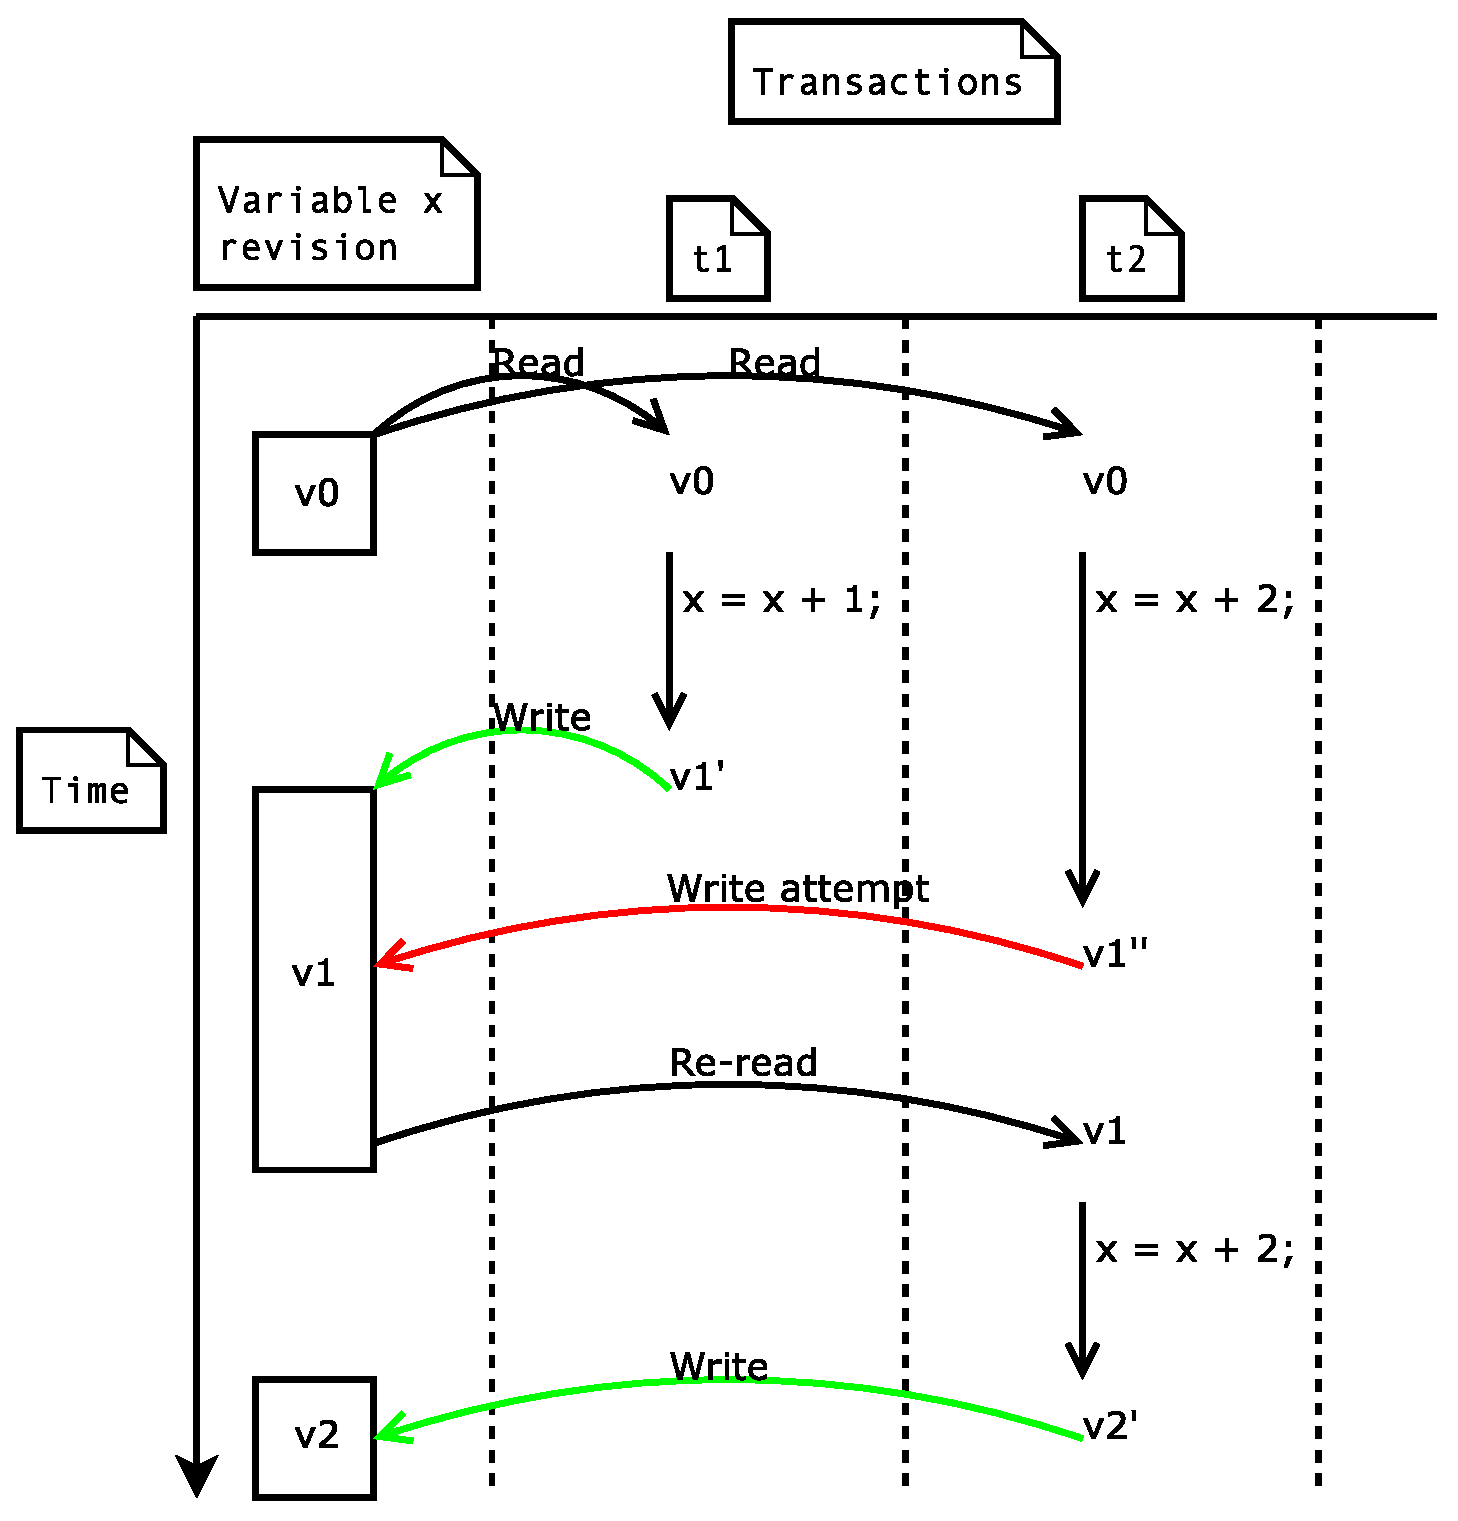
\includegraphics[scale=0.5]{\rootpath/worksheets/stm/figures/transaction}
\caption{Two transactions share memory and both have a reference to variable x. They have a racecondition, both doing calculations based on x, and writing back to x. \ac{STM} ensures that there is no lost update when t2 attempts to write, and enforces a recalculation with the new x value.}\label{fig:transaction}
\end{figure}

\subsection{Conflicts}
\label{sec:stm_conflicts}
In the context of \ac{STM} a conflict is two transactions performing conflicting operations on the same data, resulting in only one of them being able to continue\cite[p. 20]{harris2010transactional}. A conflict arises if two transactions attempt to write to the same data, or if one transaction reads the data while the other writes to it.

A \ac{STM} system taking some action to avoid a conflict is called conflict resolution\cite[p. 20]{harris2010transactional}. When two transactions conflict two options exist for resolving the conflict:\begin{inparaenum}[(1)]
\item pausing a transaction, attempting to let the other transaction finish
\item letting a transaction proceed, forcing the other transaction to abort.
\end{inparaenum} 
\subsection{Common Language Constructs}
\label{sec:stm_common_constructs}
Languages supporting \ac{STM} must encompass some language construct for specifying that a section of code should be executed as a transaction and managed by the \ac{STM} system. This basic language construct is often referred to as the \bscode{atomic} block\cite[p. 49]{harris2005composable}\cite[p. 3]{harris2003language}. The \bscode{atomic} block allows programmers to specify a transaction scope wherein code should be executed atomically and isolated as described in \bsref{sec:stm_tm_properties}. The atomic block is exemplified in \bsref{lst:stm_atomic_block}. Exactly how a transaction scope is defined, varies between \ac{STM} implementations. As an example, Clojure employs the \bscode{dosync} function as shown on line 5 in \bsref{lst:stmexample} while a library based system such as JDASTM\cite{ramadan2009committing} uses calls to \bscode{startTransaction} and \bscode{commitTransaction} methods.

\begin{lstlisting}[label=lst:stm_atomic_block,
  caption={The atomic block},
  language=Lisp,  
  showspaces=false,
  showtabs=false,
  breaklines=true,
  showstringspaces=false,
  breakatwhitespace=true,
  commentstyle=\color{greencomments},
  keywordstyle=\color{bluekeywords},
  stringstyle=\color{redstrings},
  morekeywords={atomic}]  % Start your code-block

	atomic{
		v1 = x;
		v2 = y;
		z  = v1 / v2;	
	}
       
\end{lstlisting}

\subsubsection{Conditional Synchronization}
\label{subsec:stm_conditional_synchronization}
A common task in concurrent programming is executing code whenever some event occurs. As an example consider a concurrent queue shared between multiple threads in a producer consumer setup. It will be useful to only have a consumer dequeue an item whenever one is available. Accomplishing this without the need for busy waiting would also be preferable.

In \cite{harris2005composable} Harris et al. introduce the \bscode{retry} statement for assisting in conditional synchronization within the context of \ac{STM}. The \bscode{retry} statement is explicitly placed by programmers within an \bscode{atomic} block. If a transaction encounters a retry statement during its execution it indicates that the transaction is not yet ready to run and the transaction should be aborted and retried at some later point\cite[p. 73]{harris2010transactional}. The transaction is not retried immediately but instead blocks, waiting to be awoken when the transaction is to be retried. The transaction is typically retired when one of the variables involved in the transaction is updated by another transaction\cite[p. 51]{harris2005composable}. By blocking the thread instead of repeatedly checking the condition, busy waiting is avoided.

A transaction using the \bscode{retry} statement is shown in \bsref{lst:stm_retry}. If the queue is empty the transaction executes the retry statement of line 3, blocking the transaction until it is retired at a later time.
\begin{lstlisting}[label=lst:stm_retry,
  caption={The retry statement},
  language=Java,  
  showspaces=false,
  showtabs=false,
  breaklines=true,
  showstringspaces=false,
  breakatwhitespace=true,
  commentstyle=\color{greencomments},
  keywordstyle=\color{bluekeywords},
  stringstyle=\color{redstrings},
  morekeywords={atomic, retry}]  % Start your code-block

	atomic{
		if(queue.isEmpty())
			retry;
		item = queue.dequeue();
		//process item
	}
       
\end{lstlisting}

In addition to the \bscode{retry} statement Harris et al. propose the \bscode{orElse} block. The \bscode{orElse} block handles the case of waiting on one of many conditions to be true by combining a number of transaction alternatives. The alternatives are evaluated in left-to-right order and only one of the alternatives is committed\cite[p. 52]{harris2005composable}. The \bscode{orElse} block works in conjunction with the \bscode{retry} statement to determine which alternative to execute. An example of a transaction employing the \bscode{orElse} block is shown in \bsref{lst:stm_orelse}. If an alternative executes without encountering a retry statement it gets to commit and the other alternatives are never executed\cite[p. 74]{harris2010transactional}. If an alternative however encounters a \bscode{retry} statement its memory operations are undone and the next alternative in the chain is executed\cite[p. 74]{harris2010transactional}. If the last alternative encounters a \bscode{retry} statement the transaction as a whole is blocked awaiting a retry at a later time\cite[p. 74]{harris2010transactional}.

\begin{lstlisting}[label=lst:stm_orelse,
  caption={The orElse block},
  language=Java,  
  showspaces=false,
  showtabs=false,
  breaklines=true,
  showstringspaces=false,
  breakatwhitespace=true,
  commentstyle=\color{greencomments},
  keywordstyle=\color{bluekeywords},
  stringstyle=\color{redstrings},
  morekeywords={atomic, retry, orElse}]  % Start your code-block

	atomic{
		{
			if(queue.isEmpty())
				retry;
			item = queue.dequeue();
		}orElse{
			if(queue2.isEmpty())
				retry;
			item = queue2.dequeue();
		}orElse{
			if(queue3.isEmpty())
				retry;
			item = queue3.dequeue();
		}
	}
       
\end{lstlisting}

\subsection{Zombie Transactions}
\label{subsec:zombie}
A zombie transaction is a transaction which will eventually abort, but have not yet discovered so. This happens, when a transaction has observed an inconsistent read-set\cite[p. 196]{dice2006transactional}. E.g. if a transaction reads the value of a variable, which is then updated by another transaction afterwards. This is exactly the case of \bscode{t2} in the example in \bsref{fig:transaction}.

\subsection{Level of Isolation}
\label{subsec:isolation_level}
Within the context of \ac{STM} there exist two different isolation levels: weak isolation and strong isolation. Isolation describes how parts of a system perceive transactions. The terms isolation and atomicity are used interchangeably throughout the literature\cite[p. 30]{harris2010transactional}.

With the guarantee of isolation, a transaction is perceived as one atomic step. That is, the intermediate states present during the execution of the transaction are not perceived by other parts of the systems, only the committed values become visible to other parts of the system. This always holds in the case of transactions perceiving other transactions. However, if a thread executes transactional code over some data, and another thread executes non-transactional code over the same data, the concepts of weak and strong isolation handle this differently.

In the case of strong isolation it is guaranteed that transactions are atomic with respect to non-transactional access\cite[p. 2083]{herlihy2011tm}. If any data is access both within a transaction as well as out side of a transaction the \ac{STM} implementation will ensure that the variable is accessed atomically in both cases. Guaranteeing isolation atomicity between transactional and non-transactional access comes with a performance cost\cite{herlihy2011tm}. 

Weak isolation only guarantees that transactions are atomic with respect to other transactions. That is, it is up to the programmer to ensure that non-transactional access does not interfere with transactional access. In languages with side-effects, this can be hard to ensure. To mitigate this issue, side-effects could be avoided  partly or entirely. Functional languages with \ac{STM} such as Clojure or Haskell promotes immutability and is pure in regards to side-effects. This property makes it easier to handle transactions, since there is only side-effects in relation to the transaction itself. 

\section{Concurrency Issues}
In this section we present the concurrency issues related to the use of \ac{STM}. We also relate to the concurrency issues discussed in \bsref{subsec:race_coditions} and \bsref{sec:tl_ci}.
\label{sec:stm_issues}

% Composition is possible in STM. Reference to Kaspers example about composition.
% STM compared to locks
\subsection{Race Conditions}
In a setting with shared memory and multiple threads, the risk of race conditions is present. In order to negate this risk, \ac{STM} enables the programmer to define blocks of code, that must be executed atomically. The atomicity of \ac{STM} ensures that the execution conceptually take effect instantaneous, hence no race conditions can occur between transactions. This holds for both \ac{STM} with weak and strong isolation.

As the programmer explicitly has to mark code in atomic blocks to ensure safety, the code will be prone to race conditions if this is not done correctly. Therefore the programmer still need to identify the concurrency critical regions. This holds true only for weak isolation level, as \ac{STM} with strong isolation will account for changes made outside transactions. The responsibility of marking critical regions varies in different implementations of \ac{STM}. Some implementations have special reference types, that can only be modified inside a transaction. This enforces the programmer to use transactions every time he wants to manipulate the value of the reference. An example using this approach is Clojure, which is a functional language that promotes immutability, and only allows mutable references to be manipulated in transactions. In \bsref{lst:stmexample} the variables \bscode{account1} and \bscode{account2} are references, and they can only be manipulated in the transaction block, which is named \bscode{dosync}.

\subsection{Starvation}
There is a risk for starvation when using \ac{STM}. The work of transactions gets executed optimistically, and then aborted if a conflict occurs. If the same transaction keeps getting aborted and must retry its work, it might never finish. To remedy this, different strategies exist. As described in \bsref{subsub:con_managers} a contention manager can use different strategies to ensure that transactions do not starve. 

\subsection{Exceptions in Transactions}
\label{subsec:stm:side_effects}
No straightforward approach exists to handle uncaught exceptions within a transactions\cite[p. 80]{harris2010transactional}. Should the transaction attempt to commit its current state before propagating the exception or should the transaction be aborted before the exception is propagated out of the atomic block? In \cite{harris2003language} the authors propose committing the current state of the transaction before propagating the exception. Using this approach, a transaction leaves the program in the same state as an equivalent sequential code segment would have, in the case of an uncaught exception. This approach has the property that removing or adding atomic blocks around code segments does not change how exceptions should be handled by the programmer\cite[p. 79]{harris2010transactional}.

\bsref{lst:stm_exception} presents the method \bscode{move}, which moves an object from one collection to another. This happens in an atomic block, to ensure atomicity. If the \ac{STM} system commits transactions in the case of an uncaught exception and an exception is raised while trying to add the object to the destination at line 4, the programmer must manually secure that it is re-added to the source. If not, the object will be in neither collection.

\begin{lstlisting}[label=lst:stm_exception,
  caption={Exceptions in Transaction},
  language=Java,  
  showspaces=false,
  showtabs=false,
  breaklines=true,
  showstringspaces=false,
  breakatwhitespace=true,
  commentstyle=\color{greencomments},
  keywordstyle=\color{bluekeywords},
  stringstyle=\color{redstrings},
  morekeywords={atomic, retry, orElse}]  % Start your code-block

	void move(Collection source, Collection destination, Object object){
		atomic{
			source.remove(object);
			destination.add(object);
		}
	}      
\end{lstlisting}

In \cite{harris2005exceptions} Tim Harris proposes aborting and undoing the memory operations of a transaction, in the case of uncaught exceptions. As all changes are undone, the programmer is not responsible for ensuring that the program remains in a consistent state\cite[p.3]{harris2005exceptions}\cite[p. 80]{harris2010transactional}. Consider again the example presented in \bsref{lst:stm_exception}. When an exception is raised while adding the object to the destination collection at line 4, the \ac{STM} will undo the changes made by the transaction, reinsert the object into the source collection, before the exception is propagated. Propagating the exception is however problematic as the exception contains a stack trace from code which memory operations were undone. In some cases, the exception hold references to objects that are to be removed as part of undoing the transaction. Furthermore if the exception is allocated inside the transaction, some way of maintaining the exception past the undo operation must be present. Tim Harris proposes having the \ac{STM} system catch the original exception and replace it with an exception specific to the \ac{STM} system, which is known to be free of the before mentioned issues\cite[p. 3]{harris2005exceptions}. This approach however looses the original information related to the uncaught exception.

\subsection{Irreversible Actions}
\label{subsec:stm_irreversible_actions}
Transactions in \ac{STM} require that aborted transactions do not cause effects. That is, if the value of a variable is manipulated in a transaction, and the transaction is aborted, the rest of the system should never see the variable changed. This raises a problem, since some actions are not reversible, e.g. \ac{IO} performed on a disk, or network access. These are irreversible actions, and even by not committing the result of a transaction, the transaction still affects the system. 

To handle this, precautions must be taken. There are different approaches to handle this issue. In \cite[p. 4]{harris2003language} all native methods raise a runtime exception. A native method is defined as a method using system calls. In Java context, that is when a method must leave the virtual environment of the \ac{JVM}. In \cite{harris2005exceptions} a proposal is given to make libraries using native methods implement a specific interface to enable cooperation with \ac{STM}. The idea is, that the libraries will buffer the effect, until their transaction is committed, where the \ac{STM} implementation will give a callback to the library.

Another approach is, to enable the developer to mark a function, so the \ac{STM} is aware of its side effect. In Clojure it is possible to do this with the \bscode{#IO} macro. If a function is marked, and used in a transaction, a compiletime exception will be raised.

\subsection{Contention level}
%What is contention
The amount of read and writes in a memory area can be described as a contention level\cite[p. 2084]{herlihy2011tm}. A high level of contention will cause poor performance in concurrent programs, especially in \ac{STM} since multiple transactions trying to manipulate the same memory can cause a conflict. When the contention level is high, the amount of conflicts will rise, and the work made by transactions being aborted is wasted. In \ac{TL} a high contention level will cause the threads to wait, at worst being limited to linear execution, but no work is wasted. 

Due to the performance impact of contention level, it is a significant factor in the design of \ac{STM} implementations. It is an important factor in \cite{harris2003language} and \cite{herlihy2008transactional} where specific research has been done to resolve this issue.

\section{Discussion}
\label{sec:stm_discussion}
This section describes and discusses issues related to \ac{STM}. \bsref{subsec:stm:variations_in_design} describes design alternatives related to \ac{STM} systems. \bsref{sec:stm_composability} describes how \ac{STM} can support composability by allowing transactions to be nested. Finally \bsref{sec:stm_ease_of_use} describes how ease of uses studies conducted into the area of \ac{STM}.

\subsection{Variations in \ac{STM} Design}\label{subsec:stm:variations_in_design}
Different approaches for designing \ac{STM} systems exist. Many of the approaches represent a trade off between different aspects of the system. This section describes a number of design issues as well as the trade off's they represent.

\subsubsection{Eager vs Lazy Updating}
Updating memory in a \ac{STM} implementation can be done either using: eager or lazy updating.

Eager updating updates the memory associated with a variable directly and is also referred to as in-place-updating, as updates are written into the existing memory location\cite[p. 35]{afek2011lowering}. \ac{STM} implementations using eager updating, must maintain an undo log, which stores information about any writes made within transactions. The undo log is used to undo the effects of a transaction when a transaction conflicts\cite[p. 2084]{herlihy2011tm}.

Lazy updating takes the opposite approach and writes updates to local versions of the effected data\cite[p. 2084]{herlihy2011tm}. If the transaction commits, the local changes are written to the actual memory locations, while an abort causes the local changes to be discarded.\toby[inline]{Evt. noget om at lazy updating bruger mere plads fordi vi har kopier fremfor en changelog, men at hvis der så er conflicter er det nemmere at discare kopier fremfor at skulle til at udføre en changelog.}

Eager updating allows efficient commit of transactions but makes it harder to ensure that zombie transactions see consistent state\cite[p. 2084]{herlihy2011tm}.

\subsubsection{Conflict Detection}
\label{sec:stm_conflict_detection}
The act of determining whether a conflict has occurred is called conflict detection\cite[p. 20]{harris2010transactional}. Different ways of handling conflict detection exist. Eager conflict detection detects conflicts whenever a transaction attempts to access shared data, while lazy conflict detection detects conflicts just before a transaction is about to commit by validating the transactions data access\cite[p. 21]{harris2010transactional}. A lazy conflict detection scheme discards more computations that a eager scheme while a eager conflict detection scheme may cause transaction that could have committed lazily to abort\cite[p. 21]{harris2010transactional}.

Besides lazy and eager conflict detection another distinction lies in what transactions are included when performing conflict detection. A \ac{STM} system employing tentative conflict detecting will include currently active transactions when detecting conflicts, while a system using committed conflict detection only detects conflicts with already committed transactions. Eager conflict detection is often coupled with tentative conflict detection while lazy conflict detection is often coupled with committed conflict detection\cite[p. 22]{harris2010transactional}.

Conflict detection is highly related to the concepts of pessimistic or optimistic concurrency control. In pessimistic concurrency control conflicts are detected and resolved when they happen\cite[p. 20]{harris2010transactional} while optimistic concurrency control detects and resolves conflicts some time after they occur\cite[p. 20]{harris2010transactional}.

\subsubsection{Visible vs Invisible Reads}
When reading shared data \ac{STM} implementations can either employ visible, invisible or semivisible reads.

Using visible reads a \ac{STM} transaction communicates its operations to other transactions, by registering in shared memory whenever it reads a shared variable\cite[p. 2]{lev2009anatomy}\cite[p. 2085]{herlihy2011tm}. Other transactions, which are about to write to a shared variable, can then consult the written data to identify if they are about to produce a conflict. As transactions write exactly which transaction reads a variable, the writing transaction can choose to abort the reading transactions\cite[p. 2]{lev2009anatomy}.

Using invisible reads a \ac{STM} transaction does not communicate its operations to other transactions\cite[p. 114]{imbs2012virtual}. Each transaction instead maintains per read metadata which is used to validate the transaction whenever additional reads are performed\cite[p. 2085]{herlihy2011tm}.

Visible reads have the problem of being expensive and not scaling, while invisible reads are expensive due to their need for repeated validation. As such, more recent \ac{STM} implementations instead employ the semivisible read scheme\cite[p. 2085]{herlihy2011tm}.

Semivisible reads are similar to visible reads in that transaction communicate their reads to other transactions. Instead of communicating exactly what transaction read a shared variable, a transaction simply indicates that a given variable has been read by some transaction, allowing other transaction to see that a conflict exists. A counter is maintained for each transaction indicating if any conflicts occured during its execution. Expensive validation can be avoided in the vast majority of cases by checking whether any conflicts occurred during the execution of a transaction\cite[p. 2]{lev2009anatomy}.

\subsubsection{Contention Managers}
\label{subsub:con_managers}
Some \ac{STM} implementations delegate conflict resolution to a component called a contention manager\cite[p. 2085]{herlihy2011tm}. The contention manager encapsulates the \ac{STM} implementations conflict resolution policy\cite[p. 2085]{herlihy2011tm} and ensures that the \ac{STM} systems as a whole makes progress\cite[p. 1]{guerraoui2005toward}. The decision of how a to resolve a conflict can be delegated to the contention manager. Not all \ac{STM} implementations use a contention manager, but instead abort transactions immediately\cite[38]{riegel2013software}.

The decision can be delegated to a contention manager. The contention manager encapsulates the \ac{STM} implementations conflict resolution policy\cite[p. 2085]{herlihy2011tm}.

In \cite{scherer2004contention} the authors examine a number of contention manager implementation policies. By benchmarking the a implementation of the policies the authors reveal that all policies which performed well in atleast a single test, performed abysmal in atleast one other test. So no single best contention management policy was identified.

\subsection{Composability}
\label{sec:stm_composability}
As discussed in \bsref{subsec:tl_composability} concurrent implementations based on the \ac{TL} concurrency model do not compose, mainly due to the threat of deadlocks. \ac{STM} avoids the issue of deadlocks and addresses composition by allowing transactions to be nested. The basic concept is exemplified in \bsref{lst:stm_nested_transactions}. The outer transaction defined on line 1 encloses another transaction defined on line 3.

\begin{lstlisting}[label=lst:stm_nested_transactions,
  caption={Nested transactions},
  language=Java,  
  showspaces=false,
  showtabs=false,
  breaklines=true,
  showstringspaces=false,
  breakatwhitespace=true,
  commentstyle=\color{greencomments},
  keywordstyle=\color{bluekeywords},
  stringstyle=\color{redstrings},
  morekeywords={atomic, retry, orElse, var}]  % Start your code-block

	atomic{
		x = 5;
		atomic{
			x = 10;		
		}
	}
       
\end{lstlisting}
The neesting of transactions need not be direct but can occur through method calls. \bsref{lst:stm_nested_transactions_real} a example based on transferring funds from one account to another. Here an outer transaction, defined on line 1, encloses two method calls to \bscode{withdraw} and \bscode{deposit} which are defined using transactions. The transactions are effectively nested within the outer transaction.
\begin{lstlisting}[label=lst:stm_nested_transactions_real,
  caption={Real world nested transactions},
  language=Java,  
  showspaces=false,
  showtabs=false,
  breaklines=true,
  showstringspaces=false,
  breakatwhitespace=true,
  commentstyle=\color{greencomments},
  keywordstyle=\color{bluekeywords},
  stringstyle=\color{redstrings},
  morekeywords={atomic, retry, orElse, var}]  % Start your code-block

	atomic{
		var amount = 500;
		account.withdraw(amount);
		account.deposit(amount)
	}
       
\end{lstlisting}

Three main forms of transaction nesting exist: flat nesting, closed nesting and open nesting\cite[p. 1]{kumar2011hparstm}\cite[p. 42]{harris2010transactional}. Flat nesting aborts the outer transaction if an inner transaction aborts, and commits from enclosed transactions only take effect when the outer transaction commits. Under closed nesting, aborting an enclosed transaction does not terminate the outer transaction, and commits made by the enclosed transactions become visible to the outer transaction but not transactions executed by other threads. Under open nesting, commits from enclosed transactions become visible to every other transaction and if the outer transaction aborts, results of committed enclosed transactions are not rolled back. Flat nesting is simpler to implement than closed and open nesting while open and closed nesting allow for a greater degree of concurrency, especially in cases where aborts are common\cite[p. 43]{harris2010transactional}.

%\kasper[inline]{Skal lige overveje om den skal med}
%\begin{lstlisting}[label=lst:observer_transactions,
%  caption={Observer pattern with transactions},
%  language=Java,  
%  showspaces=false,
%  showtabs=false,
%  breaklines=true,
%  showstringspaces=false,
%  breakatwhitespace=true,
%  commentstyle=\color{greencomments},
%  keywordstyle=\color{bluekeywords},
%  stringstyle=\color{redstrings},
%  morekeywords={atomic, retry, orElse, var}]  % Start your code-block
%
%	public class ValueStore implements Observable{
%
%    private int value = 0;
%    private List<Observer> observers = new ArrayList<>();
%
%    public void setValue(int newValue){
%		List<Observer> shallowCopy;        
%        atomic{
%            value = newValue;
%            shallowCopy = new ArrayList<>(observers); 
%        }
%        
%        for (Observer o : shallowCopy) {
%                o.notify(this,newValue);
%        }
%    }
%
%    @Override
%    public void register(Observer observer){
%        atomic{
%            observers.add(observer);
%        }
%    }
%
%    @Override
%    public void unregister(Observer observer){
%        atomic{
%            observers.remove(observer);
%        }
%    }
%	}
%	
%	public class ValueObserver implements Observer {
%
%    @Override
%    public void notify(Observable sender, int value){
%        sender.unregister(this);
%    }
%	}
%
%	public class Main {
%
%    public static void main(String[] args){
%        ValueStore observable = new ValueStore();
%        observable.register(new ValueObserver());
%        observable.setValue(5);
%        System.out.println("Done");
%    }
%	}
%\end{lstlisting}
\subsection{Ease of Use}
\label{sec:stm_ease_of_use}
Throughout the literature, one of the main reasons for investigating \ac{STM} as a synchronization mechanism is the claim of \ac{STM} being easier to use than locking and in particular fine grained locking. This section examines two studies into this claim.
\subsubsection{Is Transactional Programming Actually Easier}
\label{sec:stm_ease_rossbach}
In \cite{rossbach2010transactional} Rossbach et al. present a study into the ease of \ac{TM}. The study is conducted over a period of three years tasking students in an \ac{OS} class at the Texas University at Austin with producing a number of concurrent implementations using coarse grained locking, fine grained locking, monitors, and \ac{STM}. The students where to do the coarse grained implementations first, followed by either \ac{STM}, monitors or fine grained locking. Over the course of these three years a total of 237 students produced 1323 concurrent implementations. 

After finishing the implementations, students where given a questionnaire asking them to supply their time spent on designing, coding and debugging the different implementation tasks, as well as ranking the used concurrency models according to syntax and the ease with which the student could reason about the model. The survey showed that students spent more time coding implementations using fine grained locking and monitors than implementations using \ac{STM} and coarse grained locking\cite[p. 51]{rossbach2010transactional}. Furthermore students spent more time debugging implementations based on fine grained locking and monitors than implementations using coarse grained locking and \ac{STM}\cite[p. 51]{rossbach2010transactional}. Furthermore the students ranked coarse grained locking as having the best syntax and as well as being easiest to think about Course grained locking was followed by \ac{STM}, fine grained locking and monitors, in the mentioned order.

In addition to surveying students the authors examine the implementations for errors, producing a taxonomy of the errors made, as well as presenting their frequency. The examination shows that at least 50\% of students made at least one error in the fine grained locking implementations, while less than 20\% of students made an error in the \ac{STM} based implementations. A a point of critique the students where to do the coarse grained implementations first, followed by either \ac{STM}, monitors or fine grained locking. As such the students would be more familiar with the problem at hand when they where to implement subsequent solutions.

To sum up, \cite{rossbach2010transactional} shows how students find coarse grained locking easier than \ac{STM}, fine grained locking, and monitors in the mentioned order\cite[p. 54]{rossbach2010transactional}. An examination of the error rates show that students were much more likely to make mistakes in the implementations based on fine grained locking and monitors than in the implementations based on \ac{STM}\cite[p. 54]{rossbach2010transactional}. It is worth noting that the study employed two different \ac{STM} implementations and that both of these implementations have a more more complex syntax than the atomic block discussed in \bsref{sec:stm_common_constructs}\cite[p. 49]{rossbach2010transactional}. Both factors can have negatively impacted the results of the study.

\subsubsection{Does Transactional Programming Keep Its Promises}
\label{sec:stm_ease_pankratius}
In \cite{pankratius2009does} Pankratius et al. present a study comparing \ac{TM} to locking as a synchronization mechanism. The study was conducted using 12 students, divided into teams of two, and tasking them with developing a parallel desktop search engine over the course of 15 weeks. Half the teams were restricted to using locks while the other half had to employ \ac{TM}. Both implementations were restricted to using C++. The locking teams employed Pthreads\cite[p. 2]{pankratius2009does} while the \ac{TM} teams employed Intel’s STM compiler\cite[p. 3]{pankratius2009does}.

The study shows that the first team to produce a working search engine was the winning \ac{TM}\cite[p. 6]{pankratius2009does}. The team had a working prototype after 5 weeks.   The locking teams spent more time debugging due to segmentation faults\cite[p. 6]{pankratius2009does}. As with the previous study, the students where presented with a survey. The survey shows that the  winning \ac{TM} based team thought they were not progressing fast enough due to having to use transactions even though they had the first prototype and the least time spent of all teams\cite[p. 7]{pankratius2009does}. The lock based teams thought they were progressing fast even though requiring more effort than the \ac{TM} based teams\cite[p. 6]{pankratius2009does}. Expert reviews revealed that the \ac{TM} based implementations were easier to understand and required fewer parallel consructs\cite[p. 6]{pankratius2009does}. All teams, including the winning \ac{TM} team, had data races which were detected by code inspection after hand-in\cite[p. 6]{pankratius2009does}. The winning \ac{TM} team spent less time than the winning lock team and had better performance\cite[p. 23]{pankratius2009does}. All locks based teams attempted to scale by employing many locks (up to 1600) which proved difficult\cite[p. 23]{pankratius2009does}.

Two of the \ac{TM} teams used locks for parts of their implementations, one team had a producer consumer setup which was controlled by a semaphore, while another team used a lock to synchronize a section with intensive \ac{IO}\cite[p. 5]{pankratius2009does}. Pankratius et al. make the case for locking and \ac{TM} coexisting rather than excluding one another.

\section{\acs{STM} Characteristics}
\label{sec:stm_eval}
This section presents how the \ac{STM} concurrency model relates to the selected characteristics presented in \bsref{chap:char}. \andreas{Should we describe which "variant" of the model we evaluate?}

\subsection{Implicit or Explicit Concurrency}
\ac{STM} as a concurrency model build upon many of the same constructs as the \ac{TL} concurrency model. Threads are started in order to introduce concurrency, and race conditions are avoided by specifying critical regions where code should be executed as a transaction and managed by the \ac{STM} system. It is the task of the programmer to explicitly employ these constructs and as such we say that \ac{STM} employs explicit concurrency. The placement is shown in \bsref{fig:stm_char_impli_expli}.

\begin{figure}[htbp]
\centering
 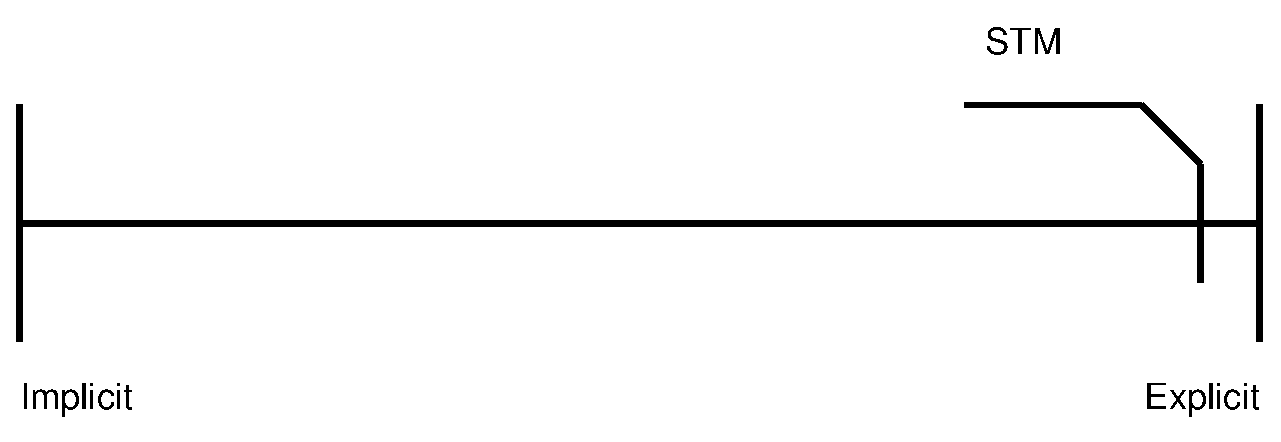
\includegraphics[width=0.9\textwidth]{\rootpath/worksheets/stm/figures/stm_char_implicit_explicit} 
 \caption{\ac{STM} on the Implicit - Explicit concurrency spectrum}
\label{fig:stm_char_impli_expli}
\end{figure}

\subsection{Fault Restrictive or Expressive Model}
\ac{STM} employs many of the principles also found in the traditional \ac{TL} approach to concurrency. Both express concurrency by starting threads and synchronising access to shared memory. While \ac{TL} gives programmers control over the low level details of synchronization, \ac{STM} delegates such work to the \ac{STM} system. Furthermore \ac{STM} limits the number of concurrency related errors which the programmer has to reason about. As such we say that \ac{STM} is an expressive concurrency model with fault restrictive elements. Because of these fault restrictive elements \ac{STM} its not consider to be truly expressive but instead resides slightly more towards the expressive extreme than the middle of the scale.\andreas{Maybe we should mention that it depends on the implementation? Some got orElse and retry, others nothing}. The placement of \ac{STM} on the fault restrictive - expressive spectrum is depicted in \bsref{fig:stm_char_fault_expressive}.

\begin{figure}[htbp]
\centering
 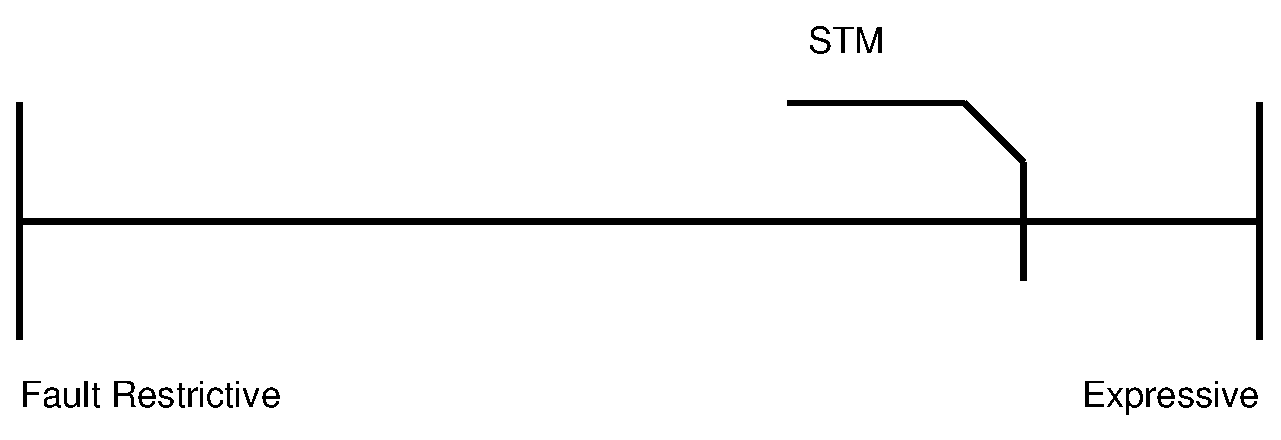
\includegraphics[width=0.9\textwidth]{\rootpath/worksheets/stm/figures/stm_char_fault_expressive} 
 \caption{\ac{STM} on the Fault Restrictive - Expressive spectrum}
\label{fig:stm_char_fault_expressive}
\end{figure}

\subsection{Pessimistic or Optimistic Model}
\ac{STM} transactions are executed concurrently, as described in \bsref{sec:stm_stm}. If the execution is successful, the transaction commits. Such an approach corresponds well with an optimistic approach to concurrency and this is also the consensus in the relevant literature. Guerraoui et al., among others, explicitly state that \ac{STM} is an optimistic model\cite[p. 1]{guerraoui2005toward}. As described in \bsnameref{sec:stm_conflict_detection}, some \ac{STM} implementations employ eager conflict detection aimed at aborting conflicting transactions as soon as possible. The overall strategy of the model however remains optimistic. As such we say that \ac{STM} is an optimistic concurrency model, with the exact placement depicted in \bsref{fig:stm_char_pes_opti}.

\begin{figure}[htbp]
\centering
 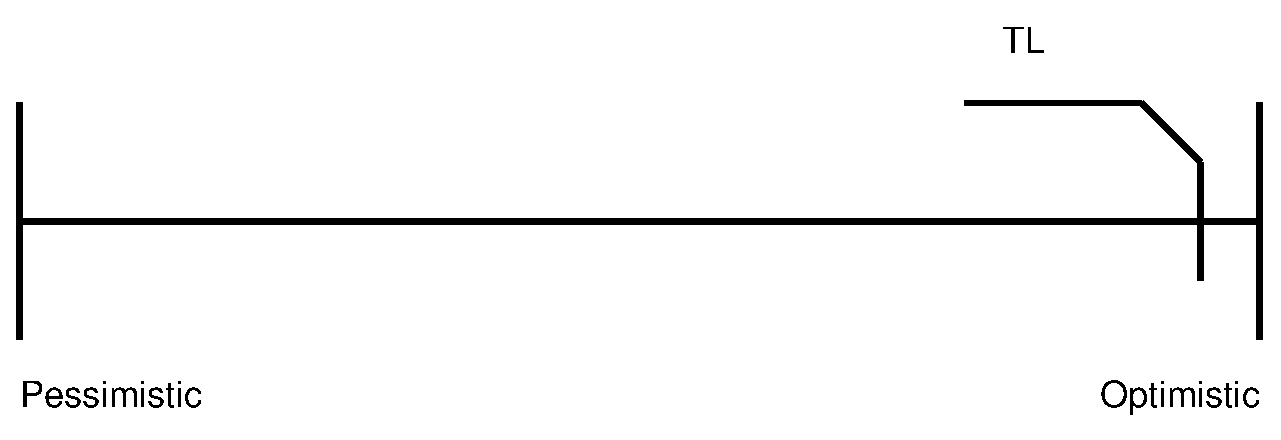
\includegraphics[width=0.9\textwidth]{\rootpath/worksheets/stm/figures/stm_char_pessimistic_optemistic} 
 \caption{\ac{STM} on the Pessimistic - Optimistic spectrum}
\label{fig:stm_char_pes_opti}
\end{figure}

\subsection{Readability and Writability}
For the reasons described in \bsref{subsec:tl_charac_read_and_write} the evaluation of the elements common to readability and writability will be presented first, followed by a presentation of the readability evaluation and the writability specific evaluations.

\subsubsection{Simplicity}
\label{subsec:stm_char_simplicity}
While \ac{STM} builds upon the shared memory also present in the \ac{TL} concurrency model it substitutes locking with memory transactions. \ac{STM} avoids the issue of deadlocks, contributing positively to its simplicity. The programmer does however still have to explicitly state when transactions are to be applied.

In \bsref{sec:stm_ease_of_use} two studies two studies into the ease of use of \ac{STM} were discussed. The first study shows that students make fewer errors using \ac{STM} than with fine grained locking. Students did however find \ac{STM} to be slightly easier than fine grained locking. Rossbach et al. note that students found the concept of transactions difficult to understand at first. The second study shows that students had a hard time predicting the performance of transactions and as a result had a hard time tuning performance.

As discussed in \bsref{subsec:stm:side_effects} and \bsref{subsec:stm_irreversible_actions}, transactions have problems composing with existing programming concepts such as \ac{IO}, exceptions and native method calls. Additional strain is put on the programmer when combining these constructs with transactions, reducing the simplicity of the model.

Based on these observations we say that \ac{STM} resides towards the high simplicity end of the low - high simplicity spectrum. While \ac{STM} addresses many of the issues that plague the \ac{TL} concurrency model, it introduces a number of new issues. These issues along with the findings in the studies discussed in \bsref{sec:stm_ease_of_use} keep \ac{STM} from having high simplicity. The exact position on low - high simplicity spectrum is depicted in \bsref{fig:stm_char_simplicity}.

\begin{figure}[htbp]
\centering
 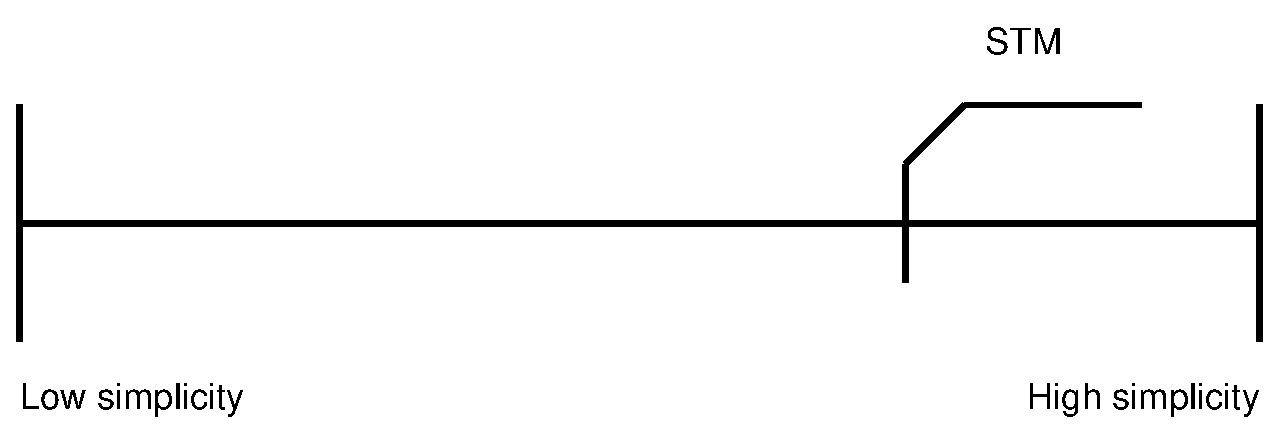
\includegraphics[width=0.9\textwidth]{\rootpath/worksheets/stm/figures/stm_char_simplicity} 
 \caption{\ac{STM} on the low - high simplicity spectrum}
\label{fig:stm_char_simplicity}
\end{figure}

\subsubsection{Orthogonality}\label{sec:stm_orthogonality}
\label{subsec:stm_orthogonality}
The \ac{STM} concurrency model consists of a few well defined\andreas{Depends, do we count retry, and orElse?} constructs: threads, communication through shared memory and synchronization using transactions. These constructs can be combined to produce concurrent implementations. As discussed in \bsref{sec:stm_composability} \ac{STM} transactions can be nested, allowing the composition of code segments employing transactions. Nested transactions allow programmers to compose large transactions from smaller transactions, much as a function can be composed from other functions. The composability problems described in \bsref{subsec:stm:side_effects} and \bsref{subsec:stm_irreversible_actions} however negatively effect the models orthogonality.

As discussed in \bsref{subsec:stm:side_effects} and \bsref{subsec:stm_irreversible_actions}, transactions have problems composing with existing programming concepts such as \ac{IO}, exceptions and native method calls. This reduces the orthogonality of \ac{STM}.

\kasper[inline]{Retry/orElse}
%In order to handle conditional synchronization the \bscode{retry} and \bscode{orElse} constructs. 

Based on these observations we say that \ac{STM} has high orthogonality limited by poor composition with some existing constructs. The position of \ac{STM} on the low - high orthogonality spectrum is shown in \bsref{fig:char_stm_orthogonality}.

\begin{figure}[htbp]
\centering
 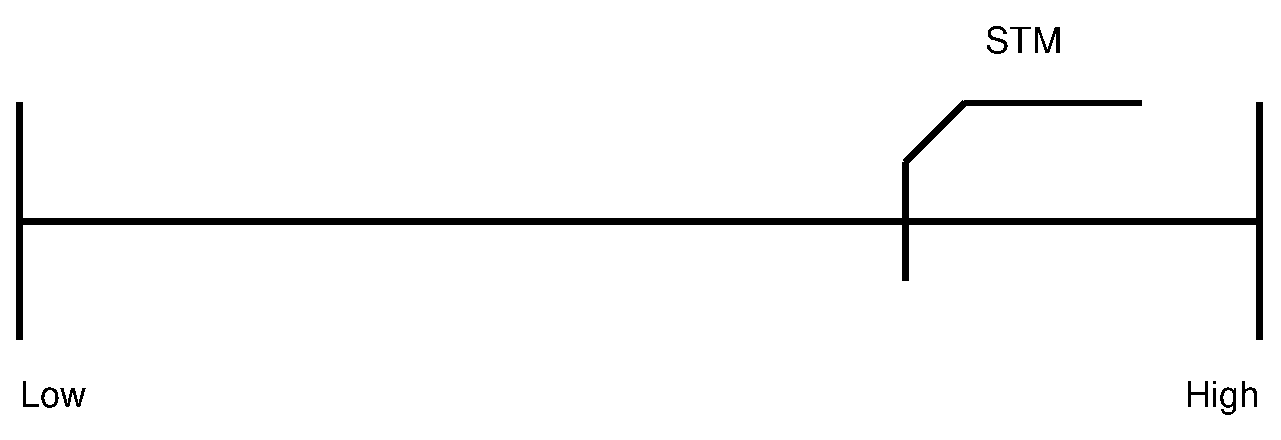
\includegraphics[width=0.9\textwidth]{\rootpath/worksheets/stm/figures/stm_char_orthogonality} 
 \caption{\ac{STM} on the low - high orthogonality spectrum}
\label{fig:char_stm_orthogonality}
\end{figure}

\subsubsection{Readability evaluation}
\kasper[inline]{Issue med numerering af referenced sektioner}
As described in \bsnameref{subsec:stm_char_simplicity} the simplicity of the \ac{STM} concurrency model resides towards the high simplicity end of the low - high simplicity spectrum. In \bsnameref{subsec:stm_orthogonality} we say that the orthogonality resides towards high end of the spectrum, limited by poor composition with existing language constructs. These results directly influence the readability of the \ac{STM} concurrency model.

The \ac{STM} concurrency model often separates the introduction of concurrency from the application of synchronization in the form of transactions. Such separation makes it harder for the programmer to reason about the implementations. However, by employing transactions the reader does not have to reason about lock ordering, which as discussed in \bsnameref{subsec:tl_char_readability} requires the programmer to reason about every code segment in which locks are employed.

The studies by Rossbach et al. and Pankratius et al., discussed in \bsref{sec:stm_ease_of_use}, show that the concept of transactions can be hard to understand at first, especially when estimating and predicting performance. Understanding the concepts of transactions is key to reasoning about synchronization using \ac{STM}, particularly when also considering the \bscode{retry} and \bscode{orElse} constructs discussed in \bsref{subsec:stm_conditional_synchronization}.

Considering these observations as well as the evaluation of simplicity and orthogonality, we say that the \ac{STM} concurrency model is slightly towards the high end of the low - high readability spectrum. While \ac{STM} addresses many of the more pressing issues found in the \ac{TL} concurrency model, it still relies on shared memory concurrency and applying synchronization to critical regions. Such a approach is prone to code fragmentation and error in identifying critical regions. Ultimately this, along with the other observations, keeps \ac{STM} from obtaining a high readability score. The exact placement of \ac{STM} on the readability spectrum is depicted in \bsref{fig:char_stm_readability}.

\begin{figure}[htbp]
\centering
 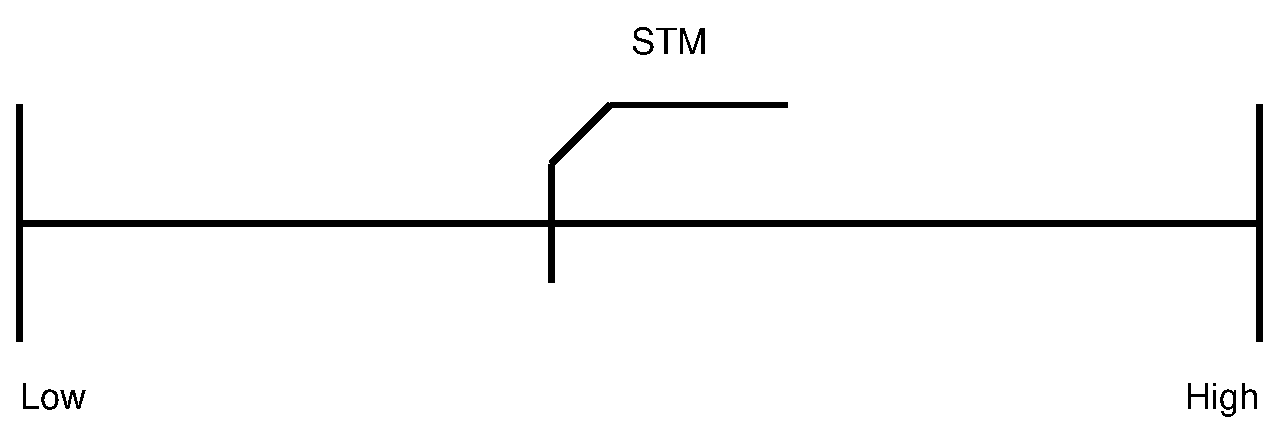
\includegraphics[width=0.9\textwidth]{\rootpath/worksheets/stm/figures/stm_char_readability} 
 \caption{\ac{STM} on the low - high readability spectrum}
\label{fig:char_stm_readability}
\end{figure}

\subsubsection{Level of abstraction}\label{sec:stm_level_of_abstraction}
\ac{STM} uses the thread model directly to support concurrency. Threads are started in order to introduce concurrency and communication is achieved via shared memory. These concepts are directly related to the \acp{OS} process/thread model described in \bsref{sec:processes_threads}.

Synchronization is accomplished using the concept of memory transactions. As described in \bsref{sec:stm_stm} and \bsref{sec:stm_common_constructs}, the programmer marks a code segment that should be executed atomically and managed by the \ac{STM} system. As such, the details of how synchronization is achieved are abstracted away. That is, transactions state that synchronization should be applied to a code segment while locking state how synchronization should be applied. The abstraction is however somewhat obstructed by transactions combining poorly with some existing language constructs, such as exceptions and \ac{IO}, as described in \bsref{subsec:stm:side_effects} and \bsref{subsec:stm_irreversible_actions}.

The employed isolation level, descried in \bsref{subsec:isolation_level}, impacts the level of abstraction provided by a given \ac{STM} implementation. Under weak isolation the programmer has to reason about non transactional code interfering with transactional code. In contrast, strong isolation abstracts this issue away and let the \ac{STM} system handle it.

While the \ac{STM} concurrency model in some aspects is close to the underlying \ac{OS} constructs, the concept of memory transactions represent a more high level approach to synchronization. Based on these observations we say that \ac{STM} resides slightly towards the low end of the level of abstraction spectrum. The exact position is depicted in \bsref{fig:char_stm_level_of_abstraction}.

\begin{figure}[htbp]
\centering
 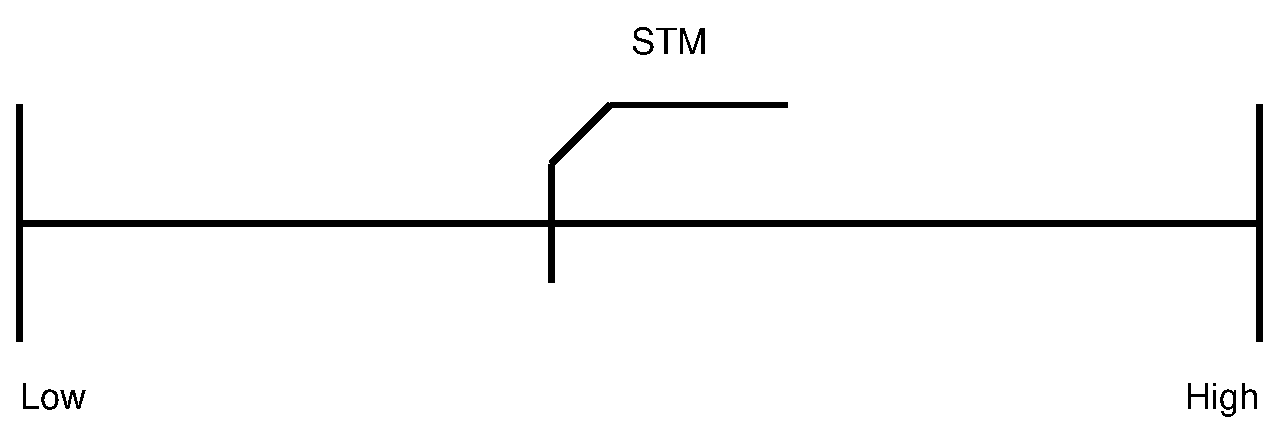
\includegraphics[width=0.9\textwidth]{\rootpath/worksheets/stm/figures/stm_char_level_of_abstraction} 
 \caption{\ac{STM} on the low - high level of abstraction spectrum}
\label{fig:char_stm_level_of_abstraction}
\end{figure}

\subsubsection{Expressivity}\label{sec:stm_expressivity}
%The level of abstraction and expressivity of a concurrency model are tightly coupled. As such the models level of abstraction also impact its expressivity. This is also the case for \ac{STM}.

\ac{STM} handles many of the issues, such as deadlocks, that plague the \ac{TL} concurrency model. Not having to reason about these issues, makes the task of expressing the intent easier. 

Transactions not combining well with existing language constructs limit the expressivity of the model. Constructs such as exceptions and \ac{IO} currently either lead to non desirable implementation strategies or are simply prohibited inside transactions. As a result the expressivity of the \ac{STM} concurrency model suffers.

\ac{STM} builds upon threads and share memory which limits its expressivity. Transactions do however represent a more declarative and expressive approach to specifying synchronization. Based on these observations we say that \ac{STM} resides slightly towards the high end of the expressivity spectrum. The exact placement is depicted in \bsref{fig:char_stm_expressivity}.

\begin{figure}[htbp]
\centering
 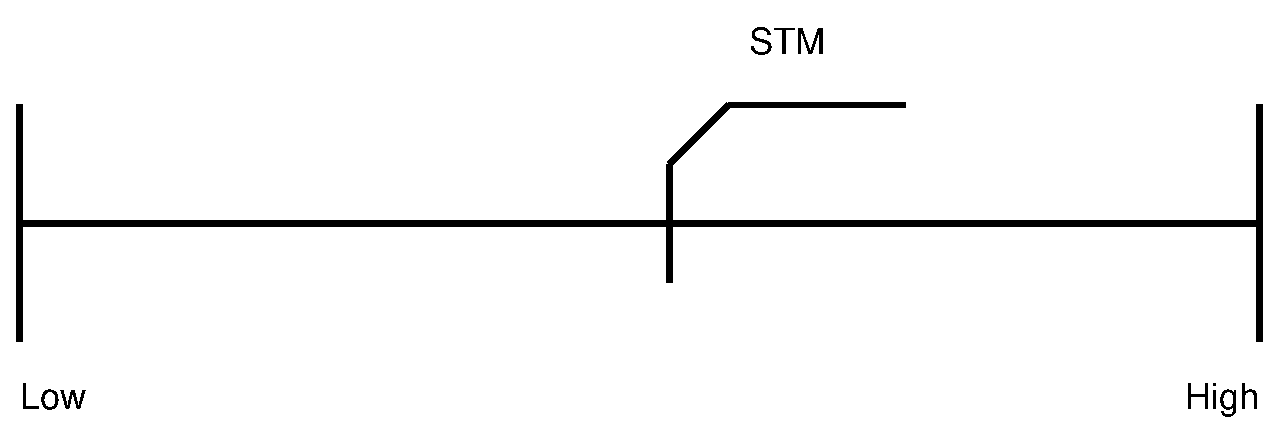
\includegraphics[width=0.9\textwidth]{\rootpath/worksheets/stm/figures/stm_char_expressivity} 
 \caption{\ac{STM} on the low - high expressivity spectrum}
\label{fig:char_stm_expressivity}
\end{figure}

\subsubsection{Writability evaluation}
\ac{STM} allows the programmer to express synchronization by stating that a code segment should be executed atomically. That is, the programmer expresses what should happen, e.g. synchronization should be applied to the code segment, as opposed to expressing how synchronization should be applied. Abstracting away the details of how synchronization is achieved allows the programmer to focus on specifying other aspects of the implementation, such as a clean design and code reuse, instead of dealing with the low level details of locking. The programmer is however not totally liberated from dealing with low level constructs as \ac{STM} still relies on threads and shared memory. Handling such low level constructs limit the models expressivity and in turn its writability.

Based on these observations, along with the evaluation of simplicity, orthogonality, level of abstraction and expressivity, we say that \ac{STM} resides slightly towards the high end of the writability spectrum. The exact position of the \ac{STM} concurrency model is shown in \bsref{fig:char_stm_writability}.

\begin{figure}[htbp]
\centering
 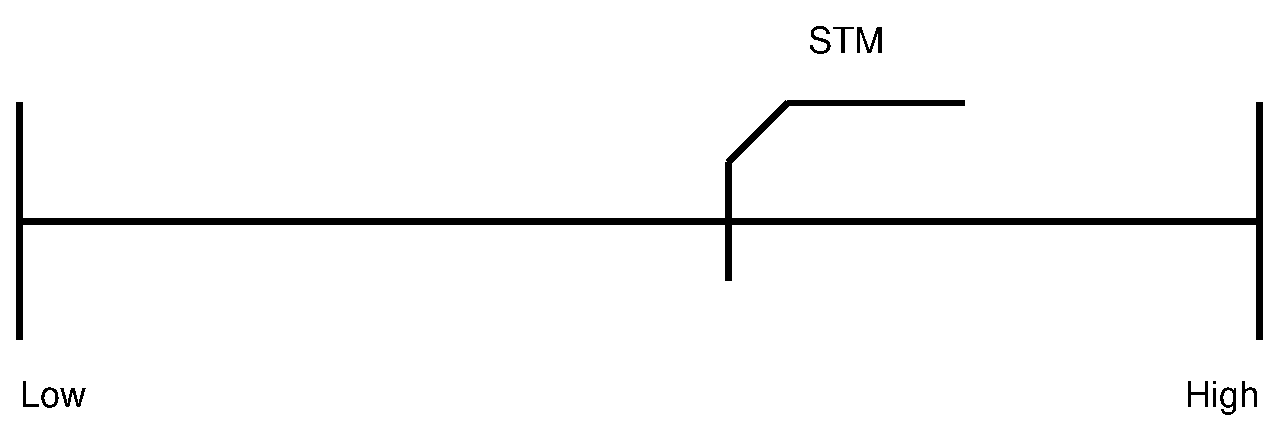
\includegraphics[width=0.9\textwidth]{\rootpath/worksheets/stm/figures/stm_char_writability} 
 \caption{\ac{STM} on the low - high writability spectrum}
\label{fig:char_stm_writability}
\end{figure}

\worksheetend
